\documentclass[11pt, twoside]{article}

\usepackage[utf8]{inputenc}
\usepackage[T1]{fontenc}
\usepackage{lmodern}
\usepackage[ngerman]{babel}
\usepackage{amsmath}
\usepackage{tabularx}
\usepackage[hyphens]{url}
\usepackage{hyperref}
\usepackage{float}
\setlength{\textfloatsep}{10pt}
\usepackage{graphicx}
\graphicspath{ {./images/} }
\renewcommand{\listfigurename}{Abbildungen}
\usepackage[margin=2.5cm, footskip=2cm]{geometry}
\usepackage[onehalfspacing]{setspace}
\usepackage{fancyhdr}
\fancyhf{}
\fancyhead[R]{Multi-Room Audio Adapter}
\fancyfoot[LE, RO]{\raisebox{2ex}{\thepage}} %Seitenanzahl im Footer
\fancyfoot[LO, RE]{
	
\includegraphics[scale=0.25]{/allgemein/htl-reutte_logo.png}
} %HTL Logo im Footer
\renewcommand{\footrulewidth}{0.4pt} %Strich über Footer
\usepackage{pdfpages}
\usepackage{enumitem}

\usepackage[style=authoryear-ibid,backend=biber]{biblatex}
\addbibresource{zitate_pi.bib}
\addbibresource{zitate_nl.bib}

% Für Darstellung des Codes im Anhang:
\usepackage{listings} % Paket für die Code-Darstellung
\usepackage{xcolor}   % Für Farbanpassungen

%\usepackage{tocbibind}

\lstset{
  basicstyle=\ttfamily\footnotesize, % Schriftart und -größe
  keywordstyle=\color{blue},         % Farben für Schlüsselwörter
  commentstyle=\color{green},        % Farben für Kommentare
  stringstyle=\color{red},           % Farben für Strings
  numbers=left,                     % Zeilennummern links
  numberstyle=\tiny\color{gray},     % Stil der Zeilennummern
  stepnumber=1,                     % Zeilennummern schrittweise erhöhen
  numbersep=5pt,                    % Abstand der Zeilennummern
  backgroundcolor=\color{white},    % Hintergrundfarbe des Code-Blocks
  frame=single,                     % Rahmen um den Code
  breaklines=true,                  % Zeilenumbruch
  showstringspaces=false,           % Leere Stellen in Strings nicht zeigen
}

\pagestyle{empty} %footer und header auf den ersten seiten nicht anzeigen

\usepackage{placeins} %statt float für figures

\usepackage{caption}
\captionsetup{justification=raggedright,singlelinecheck=false}

\usepackage{xcolor} %für das Einfügen von Farben
%Definition der Farben, für die spätere Anzeige in der Tabelle:
\definecolor{grey}{HTML}{2B2C28}
\definecolor{lightTurquoise}{HTML}{7DE2D1}
\definecolor{whiteColor}{HTML}{FFFAFB}
\definecolor{redColor}{HTML}{D90B0B}
\definecolor{lightGrey}{HTML}{3E403A}

\title{\textbf{Multi-Room Audio Adapter}}
\author{Nico Lang, Philipp Immler}
\date{Februar 2025}

\begin{document}

%\maketitle
\pagenumbering{gobble}
\newpage
\pagenumbering{arabic}

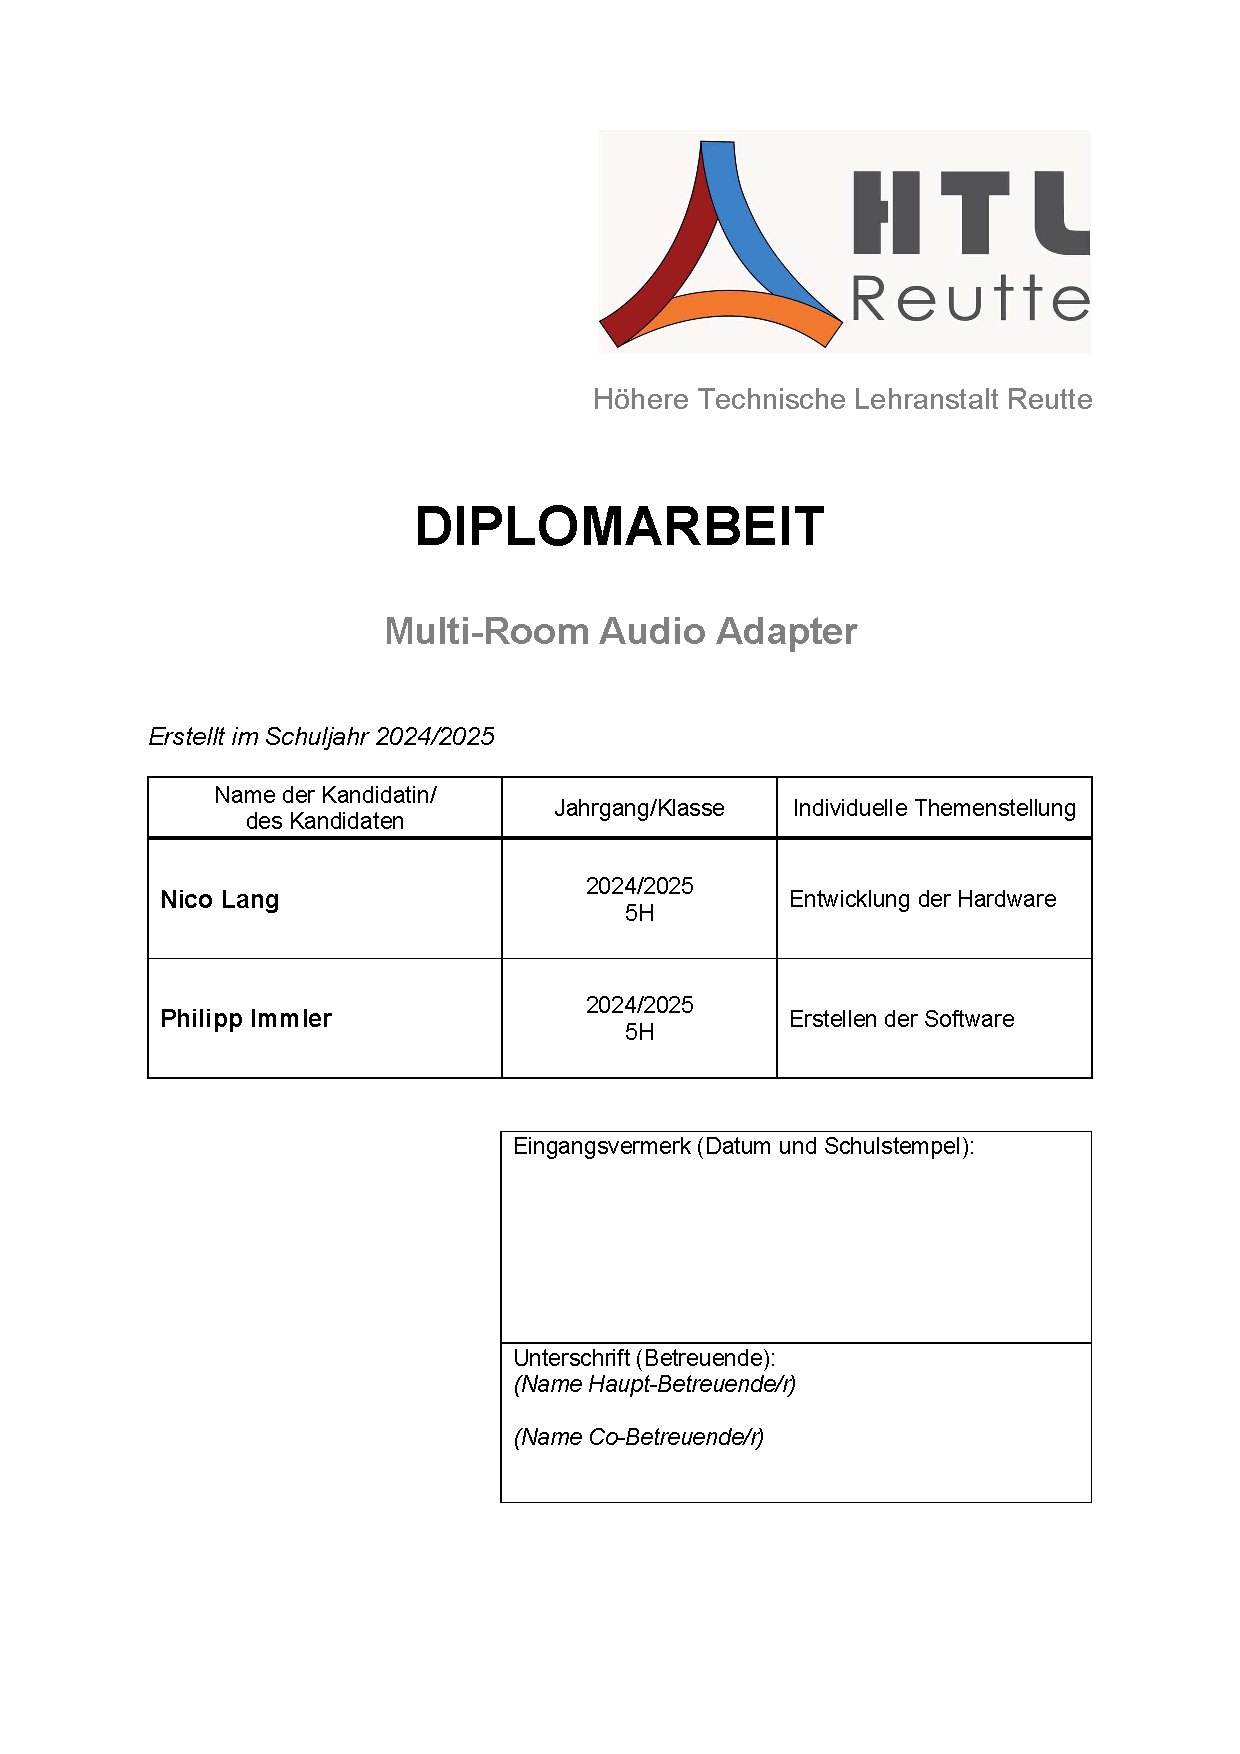
\includepdf[pages=-]{Deckblatt.pdf}

\section*{Projekt}
\subsection*{Projektteam}
\begin{figure}[H]
	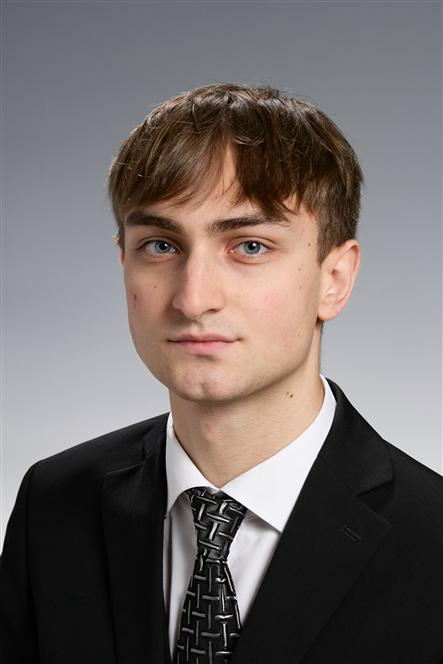
\includegraphics[scale=0.3]{/allgemein/bild_nico.jpg}
\end{figure}
\textbf{Nico Lang}\newline
Wirtschaftsingenieure/Betriebsinformatik\newline
6651 Häselgehr AT\newline
Nico.Lang@hak-reutte.ac.at\newline
\begin{figure}[H]
	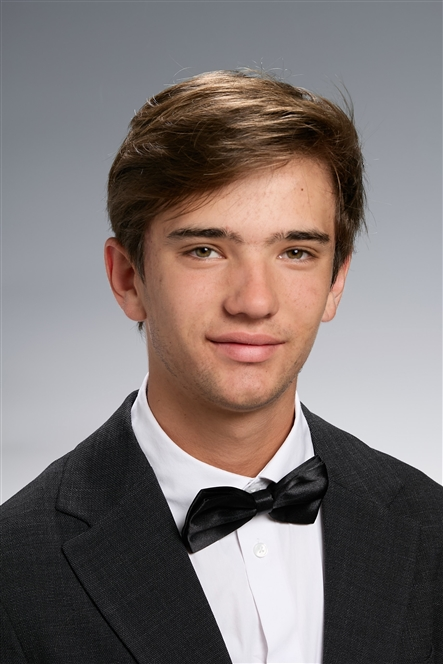
\includegraphics[scale=0.4]{/allgemein/bild_philipp.jpg}
\end{figure}
\noindent \textbf{Philipp Immler}\newline
Wirtschaftsingenieure/Betriebsinformatik\newline
6682 Vils AT\newline
Philipp.Immler@hak-reutte.ac.at

\newpage

\subsection*{Eidesstattliche Erklärung}
Hiermit versichere ich, dass ich die vorliegende Arbeit selbstständig verfasst und keine anderen Hilfsmittel als die angegebenen benützt habe. Die Stellen, die anderen Werken (gilt ebenso für Werke aus elektronischen Datenbanken oder aus dem Internet) wörtlich oder sinngemäß entnommen sind, habe ich unter Angabe der Quelle und Einhaltung der Regeln wissenschaftlichen Zitierens kenntlich gemacht. Diese Versicherung umfasst auch in der Arbeit verwendete bildliche Darstellungen, Tabellen, Skizzen und Zeichnungen. Für die Erstellung der Arbeit habe ich auch Hilfsmittel generativer KI-Tools (ChatGPT 3.5) zu folgendem Zweck verwendet: Inspiration und grobe Informationsbeschaffung. Auch Übersetzer (DeepL) wurden zur Hilfe genommen. Die verwendeten Hilfsmittel wurden vollständig und wahrheitsgetreu inkl. Produktversion und Prompt ausgewiesen.\\

\vspace{30mm}

\noindent
\begin{minipage}[c]{5cm}
	\centering \dotfill \\
	Ort, Datum
\end{minipage}
\hfill
    \begin{minipage}[c]{5cm}
        \centering \dotfill \\
        Nico Lang
    \end{minipage}
    
\vspace{25mm}

\noindent
\begin{flushright}
    \begin{minipage}[c]{5cm}
        \centering \dotfill \\
        Philipp Immler
    \end{minipage}
\end{flushright}

\newpage

\subsection*{Abstract Deutsch}
Die vorliegende Diplomarbeit beschäftigt sich mit der Entwicklung eines Multi-Room Audio Adapters (MAA). Ein einzelner Adapter besitzt dabei die Funktion, einen Audiostream aus dem Internet auf einen Line-Output auszugeben. So lassen sich die Adapter beispielsweise mit aktiven Lautsprechern per Klinkenkabel verbinden, um so Musik in voneinander getrennten Räumen abzuspielen. Welche Musik in welchem Raum spielt, ist frei konfigurierbar. Dabei erfolgt die Konfiguration per Smartphone-App. Das Endergebnis der Diplomarbeit sind somit der Adapter selbst (physischer Prototyp) und die dazugehörige Smartphone-App. \newline \\
Die Diplomarbeit lässt sich grob in die drei Teile Planung, Entwicklung und Testen/Fehlerbehebung gliedern.
\subsection*{Abstract English}
This diploma thesis deals with the development of a multi-room audio adapter. A single adapter has the function of outputting an audio stream from the Internet to a line output. For example, the adapters can be connected to active speakers via a jack cable in order to play music in separate rooms. Which music plays in which room is freely configurable. The configuration is done via smartphone app. The final result of the thesis is the adapter itself (physical prototype) and the corresponding smartphone app. \newline \\
The thesis can be roughly divided into three parts: planning, development and testing/troubleshooting.
\subsection*{Danksagung}
Wir bedanken uns bei den betreuenden Lehrpersonen Dipl. Ing. Dr. Peter L. Steger und Dipl. Päd. Johannes Köll für die kompetente Unterstützung.

\newpage
\tableofcontents
\addtocontents{toc}{\protect\setcounter{tocdepth}{0}} % Setzt den tocdepth auf 0 nur für das Inhaltsverzeichnis
\newpage
\setcounter{tocdepth}{2}  % Hiermit werden Abschnitte und Unterabschnitte im Inhaltsverzeichnis angezeigt

\pagestyle{fancy} % header und footer ab hier anzeigen
\setcounter{page}{1} %setzt den Zähler der Seiten hier auf 1

\section{Einleitung}
\begin{figure}[H]
\begin{center}
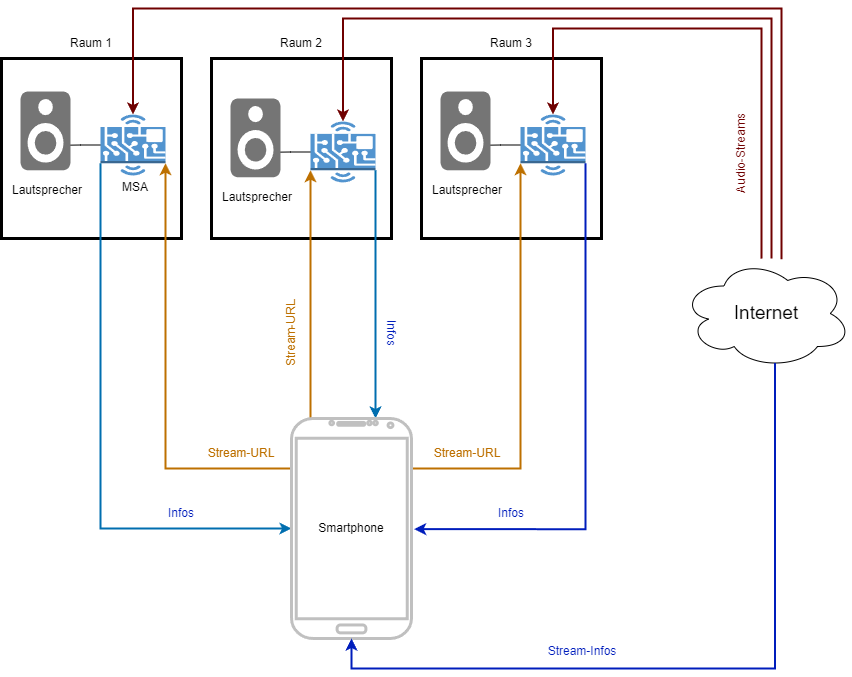
\includegraphics[width=\linewidth]{/allgemein/MAA_Konzept.png}
\caption{Skizze Gerätekette}
\end{center}
\end{figure}
Hier ist eine vereinfachte Darstellung der Gerätekette und wie sich der MAA in diese eingliedern lässt.\newline
Am unteren Bildrand ist eine Wolke mit Information dargestellt. Sie symbolisiert das Internet mit dessen Inhalt. Darüber ein Smartphone, welches mit dem Internet kommuniziert und sich so Informationen wie Stream-URLs holt und sie an den Adapter weitergibt. Der Adapter selbst (hier als blaue Platine dargestellt) holt sich den Stream selbst (also praktisch ein Audiosignal) und stellt ihn als Klinkenausgang zur Verfügung. Man kann diesen dann beispielsweise mit einem Lautsprecher verbinden und Musik hören.

\subsection{Einleitung Hardware}
Das Ziel des Hardware-Teils für folgende Diplomarbeit war, einen sinnvollen internen Aufbau des Geräts zu erzielen, die am besten geeigneten Hardware-Komponenten zu finden, das System bzw. die einzelnen Komponenten zusammenzusetzen und zu testen. Dieser Teil der Diplomarbeit wurde von Nico Lang übernommen.
Zudem beschäftigt sich dieser Teil mit dem Gehäuse des Geräts und bestimmt die technischen Anforderungen (Schnittstellen), die der Adapter letztendlich haben soll. 
Bei der Planung soll zudem darauf geachtet werden, möglichst viele Kosten einzusparen, ohne dabei die Faktoren der Sicherheit und Qualität zu vergessen.

\subsection{Einleitung Software}
Das Ziel des Software-Teils für folgende Diplomarbeit war, einerseits eine funktionierende Software für den Adapter selbst, andererseits eine funktionierende Smartphone-App zum Steuern des Adapters zu entwickeln. Dieser Teil der Diplomarbeit wurde von Philipp Immler übernommen. Die Software des Adapters wurde mit der Programmiersprache C++ codiert. Für die Entwicklung der Smartphone-App wurde TypeScript verwendet. Bei der Programmierung wurden zahlreiche Bibliotheken und Frameworks verwendet. Dies hat den Vorteil, dass diese schon vorgefertigten Code für bestimmte Probleme bieten und deshalb nicht alles von Grund auf neu entwickelt werden muss.
\section{Planung}
\subsection{Festlegung Funktionsweise}
Beim Festlegen einer grundlegenden Funktionsweise des Adapters stellen sich vor allem folgende Fragen:
\subsubsection{Was soll das System können?}
Das Hauptziel ist, dass das System in verschiedenen, voneinander getrennten Räumlichkeiten bestimmte Audiosignale auf einen Line-Ausgang abspielen kann.
\vspace{4mm}\newline
\textbf{Line-Ausgang}\newline
Ein Line-Ausgang (Line-Out) ist eine Ausgangs-Schnittstelle für analoge Audiosignale, deren Ausgangsspannung immer grob dem Line-Pegel entspricht. Dieser \glqq Line-Pegel beträgt etwa 0,5 Volt bis 1 Volt\grqq{}. \newline
Diese geringe Spannung reicht jedoch nicht, um das Audio-Signal direkt an einen Lautsprecher auszugeben. Es muss zuerst noch durch einen Verstärker verstärkt werden. Lautsprecher gibt es mit eingebautem Verstärker (aktive Lautsprecher), es gibt sie jedoch auch ohne internen Verstärker (passive Lautsprecher).
\vspace{4mm}\newline
\parencite[vgl.][]{noauthor_urlnl01_nodate}
\vspace{4mm}\newline
\textbf{Aktive vs. Passive Lautsprecher}\newline
Ein klassisches Beispiel für passive Lautsprecher sind herkömmliche Hi-Fi Stereoanlagen. Diese bestehen meistens aus einem oder mehreren Playern, einem Verstärker und zwei oder mehreren (Surround Sound also Raumklang) passiven Lautsprechern. Der Player liest das Signal (beispielsweise einer CD oder einer Schallplatte) und gibt den Line-Pegel über ein Kabel (im Hi-Fi Bereich meist Cinch oder 3,5mm Klinke) an den Verstärker weiter. Dieser Line-Pegel kann aber auch direkt aus einem TV-Gerät oder wie in unserem Fall aus einem MAA kommen. Der Verstärker verstärkt das Audiosignal nun von der geringen Spannung des Line-Pegels auf die für die Lautsprecher passende Spannung. Mit dem Lautstärkeregler am Verstärker kann man sich die Spannung (also Lautstärke) letztendlich noch auf persönliche Präferenzen anpassen. \newline
Ein Beispiel für aktive Lautsprecher sind Bluetooth-Lautsprecher, deren Hauptziel es ist, möglichst kompakt und leicht transportierbar zu sein. Solche Bluetooth-Lautsprecher enthalten im Normalfall einen Akku, um auch unterwegs, ohne aktive Stromquelle, Musik hören zu können. Somit enthält das Gehäuse den Verstärker, die Lautsprecher, den Akku und sonstige Elektronik wie unter anderem ein Bluetooth-Modul. Hier fungiert meist ein herkömmliches Smartphone als Signalgeber, ob über Bluetooth oder 3,5mm Klinke bleibt dem/der Benutzer/-in überlassen.\newline
Lenovo beschreibt Line-Ausgänge zum Beispiel folgendermaßen: \glqq Der Line-Ausgang unterscheidet sich von anderen Audioausgängen wie z. B. Kopfhörerbuchsen, da er ein Signal mit festem Pegel liefert, das nicht von der Lautstärkeregelung Ihres Geräts beeinflusst wird. Er ist für den Anschluss an Geräte gedacht, die das Audiosignal verstärken oder weiterverarbeiten können.\grqq{} \newline
Man kann also daraus schließen, dass man das Line-Out Signal des MAA vor dem Lautsprecher noch verstärken muss. Wie genau, ist dem/der Endverbraucher/-in überlassen.
\vspace{4mm} \newline
\parencite[vgl.][]{noauthor_urlnl02_nodate}
\vspace{4mm}\newline
\textbf{Audioqualität}\newline
Zudem ist es wichtig, dass das System den Ton zuverlässig und möglichst flüssig überträgt und ausgibt.\newline
\glqq Das menschliche Ohr ist theoretisch in der Lage, Frequenzen von 20 Hz bis 20 kHz zu hören. Die
Obergrenze von 20 kHz nimmt mit dem Alter ab.\grqq{} \newline
Es gibt drei wichtige Grundgrößen wenn es um Audioqualität geht: Samplerate, Auflösung und Bittiefe. Jan Baumann hat diese auf seiner Website sehr gut erklärt:
\vspace{4mm}\newline
\glqq Die \textbf{Samplerate} (Einheit Hz = Hertz) gibt an, wie oft in einer Sekunde der Audio-Pegel erfasst und gespeichert wird. Eine Angabe von 44.100 Hz (44,1 kHz) bedeutet, dass 44.100 Werte für eine Sekunde Musik gespeichert werden. Übliche Sample-Raten sind 44,1 kHz (Musik CD), 48 kHz (Film) und 96 kHz (Tonstudio).\grqq{}
\vspace{4mm}\newline
\glqq Die \textbf{Auflösung} (Einheit Bit) gibt an, wie viel Speicher für so einen Sample-Wert genutzt wird. Zum Beispiel erlauben 16 Bit (2-hoch-16) eine Skala von 65.536 Werten für jeden einzelnen Sample-Wert. Wenn wir viel Speicher für einen Wert haben, können wir das Signal also mit mehr Genauigkeit verarbeiten. Übliche Werte sind 16 Bit (Musik CD) oder 24 Bit bzw. 32 Bit im Studio.\grqq{}
\vspace{4mm}\newline
\glqq Die \textbf{Bitrate} bzw. Datenrate (kBit/s) wird oft mit der Auflösung verwechselt. Sie steht für die “Bandbreite” der Audiodatei, also welche Datenmenge in einer Sekunde verarbeitet wird. Für unkomprimierte Formate wie WAV und AIFF berechnet man die Bitrate ganz einfach, indem man die drei Werte von oben multipliziert:\grqq{}\newline
Mehr zu Audioqualität aber im Teil \glqq Auswahl interne Hardware/Digital-/Analogwandler\grqq{}
\vspace{4mm} \newline
\parencite[vgl.][]{noauthor_urlnl03_nodate}
\parencite[vgl.][]{noauthor_urlnl04_nodate}
\vspace{4mm}\newline
\textbf{Audio-Quellen}\newline
Grundsätzlich kann jeder beliebige Audiostream aus dem Internet verwendet werden. Das können beispielsweise Radiosender sein.
Ein Beispiel für einen solchen Audiostream wäre der, des österreichischen Radio-Senders \glqq OE3\grqq{}: \newline
\url{https://orf-live.ors-shoutcast.at/oe3-q2a}
\vspace{4mm}\newline
\textbf{Benutzerfreundlichkeit}\newline
Es wurde zudem viel Wert auf Benutzerfreundlichkeit gelegt. Das bedeutet, dass sich der Adapter zum einen leicht einrichten lässt, aber auch, dass er sich (mithilfe der Smartphone-App) einfach bedienen lässt.
%(vgl. (Fachbuch) \url{https://books.google.de/books?id=UI2INugaKwIC&pg=PA219#v=onepage})
\subsubsection{Was muss es nicht können?}
Dieser MAA ist als Hi-Fi Produkt für den/die klassische/n Durchschnittsbürger/in und/oder Musik-Liebhaber/innen gedacht. Aufgrund dessen wurde die Bedienung sehr einfach und benutzerfreundlich, jedoch eindeutig nicht so präzise oder vielfältig einstellbar gestaltet wie es bei professionellem Audio-Equipment der Fall ist. Während der Laie das Produkt einfach anstecken und benutzen möchte, hätte ein Audio-Nerd beispielsweise gerne noch einen eingebauten Acht-Band Equalizer und vieles mehr. Das war jedoch nicht das Ziel dieser Diplomarbeit. Es ging eher darum, die Hauptfunktion, also Ton kabellos in Räume zu übertragen, und Einstellungsmöglichkeiten per App ohne großes Kopfzerbrechen zu ermöglichen.\newline
Wie schon oben erwähnt liefert der MAA nur einen Audioausgang mit Line-Pegel und es ist ihm nicht möglich, dieses zu verstärken. Man kann also keine Kopfhörer mit einer Impedanz über 80 Ohm direkt an das Gerät anschließen (man kann theoretisch schon, aber der Ton wird sehr leise sein). Das Audiosignal muss also zuerst mit einem Verstärker verstärkt werden.\newline
\subsubsection{Wie könnte man es erweitern?}
Unsere Variante des MAA zeichnet sich vor allem durch die beliebige Erweiterbarkeit aus. In der Theorie soll es ein einzelnes Modell, also den Adapter selbst geben. Mit jedem weiteren Adapter kann dementsprechend ein weiterer Lautsprecher oder ein Raum zugefügt werden. In Zukunft wäre es auch vorstellbar, dass man aus mehreren Adaptern Gruppen bilden kann, in denen die Adapter synchronisiert sind und somit der gleiche Audiostream auf mehreren Adaptern synchron läuft. Dies ist aber technisch sehr aufwendig, da die Latenz von WiFi ziemlich hoch ist.
\subsection{Auswahl Hardwarekomponenten}
Zur Auswahl der Hardwarekomponenten des Adapters wurde zuallererst die externe Ausstattung des Adapters überlegt. Das bedeutet praktisch alles, mit dem ein Endverbraucher letztendlich zu tun hat. Dann kann der interne Teil, also die Technik dahinter, individuell auf die Anforderungen des externen Teils designet und entwickelt werden.
\subsubsection{Auswahl externe Hardware}
Der Adapter sollte ein möglichst kompakt konstruiertes und stabiles Gehäuse bekommen. An diesem ist ein einfacher Taster zur Interaktion angebracht. Mit dem Taster wurden einige Funktionen des Adapters ermöglicht. Beispielsweise per Klick, Doppelklick oder kurzem Halten. Da sich die Aufgaben des Tasters selbst gering halten (Verbindungsvorgang, Ein- und Ausschalten, ...) wurde nur ein einziger Taster verwendet, um die Komplexität des Gesamtsystems zu senken. Die weitaus komplizierteren Funktionen wurden alle samt in der Smartphone-Applikation ermöglicht. Zusätzlich wurde eine RGB-Leuchtdiode zur Statusanzeige verbaut, um beispielsweise den aktuellen Verbindungsstatus zum Mobilgerät und zum Internet anzuzeigen. \newline \\
\textbf{Gehäuse} \newline
Das Gehäuse soll alle Komponenten auf möglichst kleinem Raum zusammenhalten, schützen und kühlen. Da sich Komponenten und möglicherweise auch das Design selbst laufend änderten, wurde dieses erst gegen Ende des Projekts finalisiert. Mehr dazu im Teil "Design Adaptergehäuse". \newline \\
\textbf{Taster} \newline
Für den Taster wurde ein herkömmlicher Tactile-Button mit verlängertem Taster in das Gehäuse geplant. Auf ihm klebt eine Art Aufsatz, auf den der/die Endverbraucher/-in letztendlich drückt, um ein gleichbleibendes optisches Design des Gehäuses zu ermöglichen. Mehr dazu im Teil "Design Adaptergehäuse"\newline \\
\textbf{LED (Light-Emitting Diode)} \newline
Als Statusanzeige wurde in diesem Fall eine herkömmliche RGB-LED verwendet. Mit dieser ist es theoretisch möglich, alle Farben des RGB-Spektrums (16,7 Mio) mit einer Komponente darzustellen.\newline
Man muss sich jedoch im klaren darüber sein, für wie viel Spannung die benutzte LED gebaut ist. Dann kann man mit passenden Widerständen arbeiten, um die LED nicht aufgrund zu hoher Spannung zu beschädigen.
\vspace{4mm} \newline
\parencite[vgl.][]{noauthor_urlnl05_nodate}
\subsubsection{Auswahl interne Hardware}
\textbf{Mikrocontroller (ESP32)}\newline
Als Herz des Systems wurde ein ESP32-WROOM-32 Mikrocontroller mit angebauter Platine (DOIT ESP32 DEVKIT V1) verwendet. Der ESP32 ist ein weit verbreiteter Mikrocontroller. Das Konzept des Controllers sind GPIOs (general purpose input/output) also Pins die man mit Code mit bestimmten Funktionen beschreiben kann. Man kann die Arduino IDE mit C++ als Programmiersprache zum programmieren verwenden. Zudem verfügt er schon Onboard über einen Hybrid WIFI- und Bluetooth-Chip, wodurch externe Module vermieden, und somit Platz eingespart werden kann. Espressif selbst beschreibt den ESP32 als optimal für IoT-Anwendungen; auch wegen der hohen Energieeffizienz.\newline
Hier ein paar Grundfakten des ESP32-WROOM-32 (der Controller selbst):\newline
Der von uns benutzte ESP32 hat einen Dual-Core 32-bit Prozessor (2x Tensilica-LX6-Kernen). Der Mikrocontroller hat WLAN (802.11b/g/n) und kann ein eigenes WLAN Netzwerk (Access Point) erstellen (kleiner WebServer). Er unterstützt Bluetooth 4.0 (BLE/Bluetooth Smart) und Bluetooth Classic. Dies ist bei vielen SmartHome und IoT-Anwendungen nützlich. Er hat einen geringen Stromverbrauch von 50-70 mA (kleine Programme ohne WiFi). Der Deep-Sleep Modus macht einen Stromverbrauch von unter 0,1mA möglich. Die Anschaffungskosten fallen mit unter 10 Euro im Vergleich zu anderen Mikrocontrollern auch sehr niedrig aus.\newline
Wie schon erwähnt ist der ESP32 mit der (uns vertrauten) Arduino IDE programmierbar und kann auch in industriellen Umgebungen (-40°C bis +125°C) betrieben werden.\newline
Für den Multi Room Sound-Adapter kommt ein ESP32 Entwicklungsboard (DOIT ESP32 DEVKIT V1) zum Einsatz.\newline
Hier eine Beschreibung von Dev-Kits auf digitalewelt.at: \glqq Um alle Funktionen des ESP32 Moduls einfach nutzen zu können, gibt es sogenannte Entwicklungsboards. Diese sind nicht nur mit zusätzlichen Schaltungen für die Spannungsversorgung ausgestattet, sondern bieten uns auch die gängigen Anschlussmöglichkeiten für unsere externen Komponenten.\grqq{} \newline
Erwähnenswert ist auch, dass der ESP32 an manchen GPIOs intere Pullup- /Pulldown-Widerstände hat. \glqq Wenn man einen Pin, an dem z.B. ein Sensor hängt, mit pinMode(5, INPUT) konfiguriert, hat der Pin keinen definierten Pegel.
Aus diesem Grund kann er solange zwischen HIGH und LOW schwanken, bis ihm ein Zustand zugeschrieben wird.\grqq{} ... \glqq Dafür hat der ESP32 interne Pullup- / Pulldown-Widerstände, die zugeschaltet werden können. Diese können mit INPUT\_PULLUP als Argument im Befehl pinMode() eingeschaltet werden.
Bei INPUT\_PULLUP wird der Pin als Eingang deklariert und wenn er nicht beschaltet ist wird dieser auf HIGH gesetzt.
Bei INPUT\_PULLDOWN hingegen wird der Eingang auf LOW gesetzt.\grqq{} Pullup- /Pulldown-Widerstände sind essenziell für einen sauber konfigurierten Tactile-Button.
\vspace{4mm} \newline
\parencite[vgl.][]{noauthor_urlnl06_nodate}\newline
\parencite[vgl.][]{noauthor_urlnl07_2023}\newline
\parencite[vgl.][]{noauthor_urlnl08_nodate}
\vspace{4mm}\newline
\textbf{Digital-/Analogwandler (Audio-Modul)}\newline
Dieses Modul ist ausschlaggebend für eine gute Audioqualität. Das digitale Audiosignal vom ESP32 (Radiostream) muss nämlich für die Line-Out Buchse auf analog konvertiert werden. Dafür wird ein Modul mit dem PCM5102A (\glqq 2VRMS DirectPath™, 112 dB Audio Stereo DAC mit 32-bit, 384 kHz-PCM-Schnittstelle\grqq{}) DAC (Digital-Analog-Converter) verwendet. Auf diesem Modul befinden sich alle Komponenten sowie die Klinkenbuchse die für die Ausgabe des Audiosignals nötig sind.
\vspace{4mm} \newline
\parencite[vgl.][]{noauthor_urlnl09_nodate}
\vspace{4mm}\newline
\textbf{Akku (Li-Ion)}\newline
Das Endprodukt soll mithilfe eines Akkus auch ohne Strom auskommen, dafür wird ein Lithium-Ionen-Akku mit 3,7 Volt verwendet. Akkus dieser Art zeichnen sich durch ihre hohe Energiedichte und, unter guten Umständen, hohe Lebensdauer aus. Man verwendet Li-Ionen-Akkus meist für (tragbare) Geräte in denen andere Akkus zu schwer oder zu groß wären. \parencite[vgl.][]{noauthor_urlnl10_nodate} \vspace{4mm}\newline
Natürlich haben Li-Ionen-Akkus auch gewisse Nachteile und bergen wie jeder andere Akku Gefahren. Beispiele dafür sind elektrische Überlastung, mechanische Beschädigung und thermische Überlastung:

Eine elektrische Überlast kann etliche Gründe haben, darunter: 
\begin{itemize}
	\item Verwendung eines falschen Ladegerätes
	\item Tiefenentladung
	\item Falsche Lagerbedingungen (z.B.: zu hohe Temperaturen) 
\newline
Zitat: \glqq Hier kommt es zur Zersetzung der Elektrolytflüssigkeit und infolgedessen zur Bildung leicht brennbarer Gase. Wird anschließend versucht, die tiefentladenen Lithium-Ionen-Zellen wieder aufzuladen, kann die zugeführte Energie durch das Fehlen von Elektrolytflüssigkeit nicht mehr korrekt umgesetzt werden. Es kann zum Kurzschluss beziehungsweise zum Brand kommen.\grqq{} \parencite[][]{noauthor_urlnl11_nodate}
\end{itemize}
Eine mechanische Beschädigung jeglicher Art kann zu Kurzschlüssen im inneren der Zelle führen. Da unser Gerät nicht dafür gemacht ist, ständig in Bewegung zu sein, spielt dies keine zu große Rolle, es muss jedoch trotzdem ausreichend Schutz gegeben sein, was durch das Gehäuse sichergestellt wird.
\vspace{4mm}\newline
Wie oben schon kurz erwähnt, muss großer Wert auf die richtige Lagerung/Kühlung des Akkus gelegt werden. Wird dieser zu heiß (etwa durch den Mikrocontroller oder sonstige Bauteile) oder durch äußere Einflüsse beschädigt kann es zum Brand kommen.
\vspace{4mm}\newline
Man kann daraus schließen, dass jeder kleinste Fehler beispielsweise zu einem Brand oder sogar einer Explosion des Akkus führen kann. Es ist daher wichtig, den Akku mit absoluter Vorsicht zu handhaben. Ausreichend Tests (Betriebstemperatur, etc.), richtige Konfiguration des Ladereglers und die Auswahl des Akkus sind ausschlaggebend für die Sicherheit des Endverbrauchers und dessen Umfeld.

\parencite[vgl.][]{noauthor_urlnl11_nodate}

\textbf{Laderegler}\newline
Für einen optimalen Ladeprozess und Schutz des Akkus wird ein spezieller Laderegler verwendet. Dieser regelt somit den Ladevorgang des Akkus und hört auf zu laden, sobald dieser voll ist. Der Aufbau dieses Ladereglers ist nicht kompliziert, es gibt jeweils einen Plus- und Minuspol für den Eingang (USB-C Buchse), den Akku (im englischen auch als Battery bezeichnet) und den Ausgang.
\subsection{Anforderungen Software Adapter}
Im Folgenden wird beschrieben, welche Anforderungen an die Software des Adapters gestellt wurden: \newline \\
\textbf{Access Point} \\
Ein Access Point ist ein Gerät, welches ein WLAN (Wireless Local Area Network) aufbaut. Dabei können sich WLAN-Clients mit diesem verbinden und somit untereinander Daten austauschen. \newline
\parencite[vgl.][]{noauthor_urlpi10_nodate-1} \newline
Der Mikrocontroller soll im Konfigurationsmodus als Access Point arbeiten. Dabei wird dem/der Benutzer/in ermöglicht, sich mittels Smartphone-App mit dem Netzwerk des Mikrocontrollers zu verbinden und somit die Anmeldedaten des gewünschten Netzwerkes zu senden. Somit kann sich dann der Mikrocontroller in weiterer Folge mit dem gewünschten WLAN verbinden. Die Daten sollen dabei im JSON-Format mittels HTTP von der Smartphone-App an den Mikrocontroller gesendet werden. \newline \\
\textbf{WLAN-Client} \\
Ein WLAN-Client ist ein Gerät, welches mit einem Access Point verbunden ist und somit einen Teilnehmer in einem WLAN darstellt. Der WLAN-Client kann dabei Daten mit anderen Clients im Netzwerk austauschen. Wenn der MAA vollständig konfiguriert ist bzw. die Anmeldedaten des WLANs hat, soll sich dieser als WLAN-Client mit dem WLAN verbinden. Um den Datenaustausch zwischen Smartphone und MAA zu ermöglichen, müssen sich beide Geräte im gleichen Netzwerk befinden. Damit der MAA in weiterer Folge Audiostreams von Internetradios empfangen kann, muss zusätzlich eine Verbindung zum Internet bestehen. \newline \\
\textbf{REST-API} \\
Der Mikrocontroller soll eine REST-API bereitstellen, mithilfe der es möglich ist, per HTTP Daten mit diesem auszutauschen. Eine REST-API ist eine API, welche den Designprinzipien der REST-Architektur folgt. API steht dabei für \glqq Application Programming Interface\grqq{}. Eine API bietet im Allgemeinen eine Möglichkeit für den einheitlichen Datenaustausch zwischen Programmen. Eine REST-API (Representational State Transfer Application Programming Interface) ist dabei eine API, welche die von der REST-Architektur vorgegebenen Regeln befolgt. Sie dient  zur Kommunikation zwischen Server und Client. Der Client kann mittels HTTP Anfragen an den Server senden. Der Server liefert dann eine Antwort, welche Daten enthalten kann. \parencite[vgl.][]{noauthor_urlpi04_nodate} Auf diese Weise kommuniziert die Smartphone-App mit dem Mikrocontroller. Der Client kann dabei vordefinierte Routen aufrufen. Die aufgerufene Route bestimmt die Aktion, welche auf dem Server ausgeführt wird. Es gibt dabei verschiedene Typen von HTTP-Requests. Jeder Typ ist für eine bestimmte Aktion verantwortlich. Für die REST-API Aufrufe des MAA sind GET-, POST- und PUT-Requests möglich. Ein GET-Request wird verwendet, um Daten vom Server abzufragen. Der POST-Request wird verwendet, um neue Daten auf dem Server anzulegen. Mit einem PUT-Request werden Daten auf dem Server aktualisiert. \parencite[vgl.][]{noauthor_urlpi13_nodate} Im Folgenden werden die Routen, welche die REST-API des MAA bereitstellen soll, genauer beschrieben: \newline \\
\begin{table}[H]
\begin{tabularx}{\textwidth}{|l|l|X|}
\hline
\textbf{Route} & \textbf{Anfragen-Typ} & \textbf{Aktion} \\
\hline
/getInfo & GET & Der Server sendet die Daten: Name, MAC-Adresse, Akkustand, Lautstärke und Stream-URL im JSON-Format an den Client. \\
\hline 
/getAvailableNetworks & GET & Der Server (MAA) sendet eine Liste, welche SSID und RSSI (Stärke) von den Netzwerken, welche sich in der Reichweite von diesem befinden, im JSON-Format an den Client. Diese werden in der Smartphone-App benötigt, um auszuwählen, mit welchem Netzwerk sich der MAA verbinden soll.\\
\hline
/setConfigData & POST & Der Client sendet SSID und Passwort des Netzwerks, mit welchem sich der MAA verbinden soll, im JSON-Format an den Server. Dieser speichert dann die erhaltenen Daten in den EEPROM und startet neu.\\
\hline
/setStreamUrl & PUT & Der Client sendet die URL des Internetradios, von welchem der MAA seinen Audiostream erhalten soll, im JSON-Format an den Server. Dieser startet dann den Empfang dieses Streams und verarbeitet diesen bzw. gibt diesen in weiterer Folge auf dem Line-Out aus. \\
\hline
/setVolume & PUT & Der Client sendet die gewünschte Lautstärke (zwischen 0\% und 100\%) des Audios an den Server. Dieser setzt dann den Gain (Verstärkung) des Audio-Signals auf einen Wert zwischen 0 und 1. \\
\hline
/pauseStream & POST & Wenn dieser Request an den Server gesendet wird, stoppt dieser den aktuellen Audiostream. \\
\hline
/continueStream & POST & Beim Empfang dieses Requests setzt der Server den gestoppten Audiostream fort. \\
\hline
\end{tabularx} 
\caption{REST-API Routen}
\end{table}
\noindent
\textbf{Audiostreaming} \\
Der Mikrocontroller sollte in der Lage sein, Audiostreams aus dem Internet zu empfangen, diese zu dekodieren und die dekodierten Daten als Signale auf dem Line-Out auszugeben. Dabei beschränken wir uns am Anfang auf Streams im MP3-Format, welches am häufigsten verwendet wird. Bei einem HTTP-Audiostream wird ein Audiofile in mehrere kleine Stücke zerteilt, welche dann per HTTP an den Client gesendet werden. Dieser fügt diese Stücke dann wieder zu einem Audiofile zusammen. Die MP3-kodierten Audiodaten müssen dann in weiterer Folge in ein PCM(Pulse Code Modulation) - Signal dekodiert werden, welches dann von dem Digital-Analog-Wandler in ein analoges Audiosignal umgewandelt wird. Das analoge Audiosignal kann dann auf der Lautsprecherbox ausgegeben werden.
\subsection{Anforderungen Smartphone-App}
Es wurde festgelegt, dass die Smartphone-App die folgenden Funktionalitäten bereitstellen soll:
\vspace{4mm}\newline 
\textbf{Verwaltung von Adaptern}  \\
Mit der App soll es einerseits möglich sein, neue Adapter zu konfigurieren, andererseits bereits hinzugefügte Adapter zu verwalten. Dabei können von den Adaptern Daten, wie beispielsweise MAC-Adresse und Akkustand, angezeigt werden. Außerdem soll regelmäßig überprüft werden, ob die Adapter vom Smartphone aus erreichbar sind.
\vspace{4mm}\newline
\textbf{Verwaltung von Radiostationen} \\
Es sollte zudem möglich sein, nach Audiostreams von Internetradios zu suchen und diese einer persönlichen Favoritenliste hinzuzufügen.
\vspace{4mm}\newline
\textbf{Verwaltung von Verbindungen} \\
In weiterer Folge soll es möglich sein, Verbindungen zwischen Adaptern und Internetradio-Streams herzustellen und diese zu verwalten. Dabei soll der Stream gestoppt und fortgesetzt werden können und die Lautstärke der Audio-Ausgabe des MAA einstellbar sein.
\vspace{4mm}\newline
\textbf{Speicherung von Benutzerdaten} \\
Letztendlich soll es noch möglich sein, sich als Benutzer/in anzumelden bzw. zu registrieren und Benutzerdaten, wie Favoritenliste und hinzugefügte Adapter, welche in der Cloud gespeichert sind, abzurufen. Die Speicherung in der Cloud hat dabei den Vorteil, dass der/die Benutzer/in sich auf jedem beliebigen Gerät mit seinen/ihren Anmeldedaten anmelden und somit seine/ihre Daten abrufen kann.
\subsection{Auswahl Technologien}
\subsubsection{Protokolle}
In diesem Kapitel geht es um die Recherche und Auswahl von Protokollen, die für den Datenaustausch verwendet wurden.
Protokolle werden in der Informatik im Allgemeinen verwendet, um eine standardisierte Kommunikation zwischen zwei oder mehreren Geräten zu ermöglichen. Diese standardisierte Kommunikation wird durch das Festlegen von Standards und Normen erreicht. \parencite[vgl.][]{noauthor_urlpi16_nodate}
\newline \\
\textbf{HTTP} \\
Das \glqq Hyper Text Transfer Protocol\grqq{} ist eines der weitverbreitetsten Protokolle im Web und wird größtenteils für die Kommunikation zwischen Browsern und Webservern eingesetzt. Dabei basiert es grundlegend auf Anfragen (Requests) und Antworten (Responses). Wenn also z.B. ein Client einen HTTP-Request (Anfrage) an einen Server sendet, antwortet dieser im Idealfall mit einer HTTP-Response (Antwort). Das HTTP-Protokoll basiert auf dem TCP/IP-Protokoll, auf welches aber in dieser Diplomarbeit nicht genauer eingegangen wird. In der Diplomarbeit wurde HTTP einerseits für die Kommunikation zwischen Smartphone-App (Client) und Mikrocontroller (Server) mittels REST-API und andererseits zum Streamen der Audio-Daten aus dem Internet verwendet. \parencite[vgl.][]{noauthor_urlpi01_2020}
\newline \\
\textbf{mDNS} \\
Das Multicast Domain Name Service - Protokoll hilft in kleineren, lokalen Netzwerken bei der Namensauflösung. Im Web dominiert das bekanntere DNS (Domain Name Service) - Protokoll. Dieses dient dazu, die IP-Adresse hinter einer Domain zu ermitteln. Dabei gibt es einen DNS-Server, welcher eine Art  Liste führt, in der aufgeführt ist, welcher Domainname zu welcher IP-Adresse gehört. Wenn man also im Browser eine URL eingibt, stellt der Client dem DNS-Server eine Anfrage, welche den Domainnamen der angefragten URL beinhaltet. Dieser sendet anschließend die zugehörige IP-Adresse zurück, mit der sich der Client dann verbindet. Dieser Ansatz ist allerdings in kleineren, lokalen Netzwerken eher unpraktisch, da ein eigener Server benötigt wird. Als Alternative dazu dient das sogenannte mDNS -Protokoll, welches mit Multicast arbeitet und daher keinen DNS-Server benötigt. Beim Multicast sendet ein Teilnehmer eines Netzwerks eine Nachricht an mehrere Teilnehmer im Netzwerk. Bei mDNS fragt also das Gerät, welches sich mit einem anderen Gerät verbinden will, andere Geräte im Netzwerk, ob der entsprechende Domainname zu diesen gehört. Wenn dies der Fall ist, meldet sich das zugehörige Gerät und somit lässt sich eine Verbindung mit diesem herstellen. \parencite[vgl.][]{noauthor_urlpi19_2022} In der Diplomarbeit wird mDNS verwendet, um eine Verbindung mit den MAA aufzubauen. Der Hostname eines MAA setzt sich dabei aus \glqq MAA\grqq{} und den letzten drei Byte der MAC-Adresse, getrennt durch einen Unterstrich, zusammen. Dies macht deshalb Sinn, weil somit jeder MAA einen eindeutigen Namen bekommt, da die letzten drei Byte einer MAC-Adresse eines jeden Netzwerkgerätes weltweit eindeutig sind. Die IP-Adresse der MAA kann nicht zur eindeutigen Identifizierung dieser verwendet werden, da in den meisten Netzwerken ein DHCP (Dynamic Host Configuration Protocol) - Server vorhanden ist, der die IP-Adressen automatisch vergibt. Deshalb ändert sich diese ständig. Die MAC-Adresse hingegen bleibt immer gleich. \parencite[vgl.][]{noauthor_urlpi20_nodate} Mithilfe von mDNS ist jeder Adapter unter seinem Namen gefolgt von \glqq .local\grqq{} auffindbar. Ein Adapter mit dem Namen \glqq MAA\_3C4D5E\grqq{} ist also im lokalen Netzwerk unter \glqq MAA\_3C4D5E.local\grqq{} auffindbar.
\newline \\
\textbf{I2S}\\
Das \glqq Inter IC Sound Protocol\grqq{} wird verwendet, um Stereo-Audio-Daten zwischen ICs (Integrated Circuits) auszutauschen. Es ist dabei zu unterscheiden von dem I2C (Inter-integrated circuit) - Protokoll, welches rein für den Datenaustausch zwischen ICs verwendet wird und somit nicht für Audiodaten spezialisiert ist. Für die Datenübertragung benötigt das I2S-Protokoll folgende Leitungen:
\begin{itemize}
	\item Taktleitung
	\item Wortauswahl
	\item mindestens eine Datenleitung
\end{itemize}
Die Datenübertragung erfolgt seriell und synchron. Das heißt, dass die Daten nacheinander durch eine Leitung (die Datenleitung), in einem bestimmten Takt, welcher von der Taktleitung vorgegeben wird, übertragen werden. Wenn Audiodaten im Stereo-Format (linker und rechter Kanal) übertragen werden, wählt die Wortauswahl-Leitung jeweils den Kanal aus, welcher übertragen werden soll. \parencite[vgl.][]{noauthor_urlpi12_nodate} \\
In der Diplomarbeit wurde das I2S Protokoll verwendet, um die digitalen Stereo-Audio-Daten vom Mikrocontroller an den Digital-Analog-Wandler zu übertragen. Dabei werden die Buffer, die der Mikrocontroller vom Audiostream erhält, mittels I2S an den Digital-Analog-Wandler gesendet, welcher die digitalen Daten in analoge PCM (Pulse Code Modulation) Daten umwandelt, sodass diese dann anschließend auf der Lautsprecherbox ausgegeben werden können. Dabei wurden folgende Parameter für die Datenübertragung gewählt:
\begin{itemize}
	\item Bittiefe: 16 Bit pro Sample
	\item Audio-Kanäle: 2
	\item Sample-Rate: 44100 kHz
\end{itemize}
\subsection{Auswahl Softwaretools}
In diesem Kapitel geht es um die Recherche und Auswahl von geeigneten Softwaretools, welche für die App-Entwicklung, als auch für die Entwicklung der Software des Mikrocontrollers verwendet wurden. Des Weiteren werden auch noch die Tools beschrieben, welche für das Schreiben der Diplomarbeit verwendet wurden.
\subsubsection{Softwaretools zum Schreiben der Diplomarbeit}
Im Folgenden werden die Softwaretools, welche zum Schreiben der Diplomarbeit benutzt wurden, aufgezählt und beschrieben.
\vspace{4mm}\newline
\textbf{\LaTeX} \\
"LaTeX ist ein hochwertiges Schriftsatzsystem, das Funktionen für die Erstellung technischer und wissenschaftlicher Dokumentationen enthält. LaTeX ist der De-facto-Standard für die Kommunikation und Veröffentlichung von wissenschaftlichen Dokumenten." \parencite{noauthor_urlpi29_nodate} \\
LaTeX wurde für die Diplomarbeit gewählt, weil es sich sehr gut für das Schreiben von wissenschaftlichen Arbeiten, vor allem mit technischem Bezug, eignet und wir somit schon damit vertraut sind, wenn wir es in Zukunft, z.B. im Studium, benutzen müssen.
\vspace{4mm}\newline
\textbf{draw.io}
"draw.io ist eine kostenlose Online-Diagrammsoftware zur Erstellung von Flussdiagrammen, Prozessdiagrammen, Organigrammen, UML, ER und Netzwerkdiagrammen." \parencite{noauthor_urlpi30_nodate} \\
Alle Diagramme, welche in der Diplomarbeit zu sehen sind, wurden in draw.io erstellt, weil es einfach zu handhaben ist und eine sehr große Auswahl an Diagrammtypen und Formen bereitstellt.
\vspace{4mm}\newline
\textbf{Visual Studio Code} \\
"Visual Studio Code ist ein leichtgewichtiger, aber leistungsstarker Quellcode-Editor, der auf Ihrem Desktop läuft und für Windows, macOS und Linux verfügbar ist. Er bietet integrierte Unterstützung für JavaScript, TypeScript und Node.js und verfügt über ein umfangreiches Ökosystem von Erweiterungen für andere Sprachen und Laufzeiten (wie C++, C\#, Java, Python, PHP, Go, .NET)." \parencite{noauthor_urlpi31_nodate} \\
Visual Studio Code wurde als IDE für den Code der Diplomarbeit gewählt, weil durch die unzähligen Erweiterungen viele verschiedene Programmiersprachen und Bibliotheken unterstützt werden und somit der gesamte Code, sowohl für den Mikrocontroller als auch für die Smartphone-App, darin geschrieben werden konnte.
\vspace{4mm}\newline
\textbf{GitHub} \\
Git im Allgemeinen ist das meistverbreitete Versionskontrollsystem. Ein Versionskontrollsystem wird verwendet, um den Versionsverlauf einer Software zu erfassen. Dies hat den Vorteil, dass man bei auftretenden Fehlern jederzeit wieder auf eine ältere Version der Software umsteigen kann. Ein weiterer Vorteil beim Einsatz eines Versionskontrollsystems ist, dass mehrere Entwickler gleichzeitig an derselben Software arbeiten können. Git gehört zu den DVCS (Distributed Version Control Systems), also verteilten Versionskontrollsystemen. Das heißt, dass der Versionsverlauf der Software nicht zentral auf einem Server gespeichert ist, sondern auf den Rechnern der Benutzer, in einem sogenannten Repository. Dies bietet höhere Sicherheit, Performance und Flexibilität. \parencite[vgl.][]{atlassian_urlpi17_nodate} \\ 
GitHub ist eine Software, die Git verwendet. Dabei ist Github cloud-basiert, das heißt, es ist online zugänglich und benötigt deshalb keine eigene Software auf dem Rechner. Außerdem hat Github  eine sehr benutzerfreundliche Oberfläche, was es auch für Einsteiger leichter verständlich macht. \parencite[vgl.][]{noauthor_urlpi18_nodate}
In der Diplomarbeit wurde GitHub für die Verwaltung des Codes und der Dokumente verwendet. Der Vorteil dabei ist, dass jedes Projektmitglied auf seinem lokalen PC an den Dokumenten arbeiten kann und die Änderungen dann per GitHub synchronisiert werden können.
\vspace{4mm}\newline
\textbf{DeepL} \\
Bei DeepL handelt es sich um einen Übersetzer, der KI einsetzt und somit einer der genauesten Übersetzer weltweit ist. DeepL wurde aufgrund seiner Genauigkeit und kostenlosen Verfügbarkeit in der Diplomarbeit verwendet, um englische Texte ins Deutsche zu übersetzen.
\subsubsection{Bibliotheken Mikrocontroller}
Im Folgenden werden die Bibliotheken, welche für die Programmierung der Mikrocontroller-Software verwendet wurden, aufgezählt und beschrieben.
\vspace{4mm}\newline
\textbf{Arduino Core} \\
(https://github.com/espressif/arduino-esp32) \\
Die \glqq Arduino-Core\grqq{}-Bibliothek wurde verwendet, um den ESP32 ähnlich wie ein Arduino-Board programmieren zu können. Es erleichtert dabei die Programmierung enorm. Vor allem dann, wenn man schon Vorerfahrung mit der Programmierung von Arduino-Boards hat. Ein weiterer Vorteil ist, dass diese Bibliothek bereits weitere nützliche Bibliotheken beinhaltet, welche für die Programmierung benötigt werden.
\vspace{4mm}\newline
\textbf{WiFi} \\
(https://github.com/espressif/arduino-esp32/tree/master/libraries/WiFi) \\
Die\grqq{} WiFi\grqq{}-Bibliothek ist eine offizielle Bibliothek von Arduino, welche in der\grqq{} Arduino-Core\grqq{}-Bibliothek inkludiert ist. Sie wird verwendet, um die Funktionen der eingebauten Wi-Fi-Antenne des ESP32 zu nutzen. Der ESP32 kann dabei entweder als Access Point oder als Client fungieren. Wenn er als Access Point fungiert, stellt er ein eigenes Wi-Fi-Netzwerk bereit, mit dem sich andere Geräte verbinden können und der ESP32 somit einen Host darstellt. Als Client kann er sich mit anderen Wi-Fi-Netzwerken bzw. Access Points verbinden. In der Diplomarbeit fungiert der ESP32 sowohl als Access Point, als auch als Client. \parencite[vgl.][]{noauthor_urlpi24_nodate}
\vspace{4mm}\newline
\textbf{ArduinoJson} \\
(https://github.com/bblanchon/ArduinoJson) \\
Die \glqq ArduinoJSON\grqq{}-Bibliothek wird verwendet, um Daten in das JSON-Format zu codieren. JSON (Java Script Object Notation) ist ein Datenformat, welches  für den einheitlichen Datenaustausch zwischen Servern und Clients verwendet wird. Dabei verwendet JSON sogenannte Schlüssel-Wert-Paare. Das heißt, einem Wert ist immer ein eindeutiger Schlüssel zugeordnet. In der Diplomarbeit realisiert die \glqq ArduinoJSON\grqq{}-Bibliothek den einheitlichen Datenaustausch zwischen Webserver (ESP32) und Client (Smartphone). \parencite[vgl.][]{noauthor_urlpi11_nodate}
\vspace{4mm}\newline
\textbf{WebServer} \\
Die \glqq WebServer\grqq{}-Bibliothek wird verwendet, um einen Webserver auf dem ESP32 bereitzustellen. Dieser ist in Kombination mit der REST-API wichtig für den Datenaustausch zwischen MAA und Smartphone-App. Auf die REST-API wurde bereits im Kapitel 3.3 genauer eingegangen. Der Webserver kann Anfragen von Clients entgegennehmen und diesen Antworten zurücksenden. Dabei gibt es vordefinierte Routen, welche aufrufbar sind.
\vspace{4mm}\newline
\textbf{ESP8266Audio} \\
(https://github.com/earlephilhower/ESP8266Audio) \\
Die \glqq ESP8266Audio\grqq{}-Bibliothek wurde ursprünglich für das Vorgängermodell des ESP32, den ESP8266, entwickelt. Sie wurde allerdings mittlerweile von den Entwicklern angepasst, sodass man sie auch für den ESP32 verwenden kann. Die Bibliothek stellt Funktionen zum Empfangen, Dekodieren und Ausgeben von Audio-Daten bereit. Die Bibliothek wurde in der Diplomarbeit verwendet, um MP3-Streams vom Internet zu empfangen, diese zu dekodieren und die dekodierten PCM-Signale über I2S an den DAC zu senden. Der ESP32 verfügt zwar bereits standardmäßig über Funktionen, mit deren Hilfe man Audiodaten mittels I2S übertragen kann, allerdings sind diese sehr komplex in der Verwendung und Konfiguration. Da die \glqq ESP8266Audio\grqq{}-Bibliothek bereits die perfekte Lösung für die Anforderungen der Mikrocontroller-Software bietet, wurde deshalb diese verwendet. \newline \\
\textbf{Preferences} \\
(https://github.com/espressif/arduino-esp32/tree/master/libraries/Preferences) \\
Die \glqq Preferences\grqq{}-Bibliothek wird verwendet, um Schreib- und Lesezugriffe auf den eingebauten EEPROM (Electrical Eresable Programmable Read Only Memory) des ESP32 durchzuführen. Dabei werden die im EEPROM gespeicherten Werte mittels eindeutiger Schlüssel identifiziert.
\subsubsection{Softwaretools Smartphone-App}
\textbf{TypeScript} \\
Bei TypeScript handelt es sich um eine Erweiterung von JavaScript. Der Vorteil von TypeScript ist, dass dieses eine statische Typisierung ermöglicht. Reines JavaScript hat eine dynamische Typisierung. Das heißt, dass den definierten Variablen erst durch den Interpreter ein konkreter Datentyp zugewiesen wird. Im Gegensatz dazu, kann man in TypeScript den Variablen direkt konkrete Datentypen zuweisen. Dadurch wird eine höhere Typensicherheit und eine bessere Wartbarkeit des Codes garantiert. \parencite[vgl.][]{noauthor_urlpi32_2023} Aufgrund dieser Vorteile wurde TypeScript in der Diplomarbeit verwendet. 
\vspace{4mm}\newline
\textbf{Node.js} \\
Bei Node.js handelt es sich um eine JavaScript-Laufzeitumgebung, welche es ermöglicht, JavaScript-Code und somit auch TypeScript-Code lokal auf dem Rechner auszuführen. Normalerweise ist JavaScript eine Programmiersprache, welche für die Frontend-Entwicklung eingesetzt wird und nur im Browser läuft. Mit der Verwendung von Node.js ist es allerdings möglich, JavaScript auch im Backend, also lokal auf dem Rechner, zu verwenden. Node.js stellt außerdem einen eigenen Paket-Manager namens \glqq npm\grqq{} (Node Package Manager) bereit, der es ermöglicht, zahlreiche Open-Source-Pakete, für unterschiedlichste Anwendungen zu installieren. Somit können mithilfe von Node.js die Vorteile, welche JavaScript bietet, zur Entwicklung zahlreicher Apps verwendet werden. \parencite[vgl.][]{noauthor_urlpi25_2021}
Node.js wurde in der Diplomarbeit verwendet, um die Entwicklung mit React Native bzw. Expo zu ermöglichen.
\vspace{4mm}\newline
\textbf{React Native} \\
React Native ist ein Framework, welches die plattformübergreifende Entwicklung von Apps ermöglicht. Das heißt, man schreibt einen Code in JavaScript bzw. TypeScript und kann aus diesem dann eine IOS-, Android- oder Web-App bauen. Um eine React Native App auszuführen, wird die Node.js-Laufzeitumgebung benötigt, welche im vorherigen Teil beschrieben wurde. React Native wurde erstmals 2015 von Meta (damals noch Facebook) als Open-Source-Projekt veröffentlicht. Seither wird es weiterhin von Meta gewartet bzw. weiterentwickelt und hat eine riesige Community, welche ständig neue Bibliotheken für das Framework veröffentlicht. React Native basiert auf React, welches man bereits aus der Webentwicklung kennt. Der Vorteil von React im Gegensatz zur normalen Webentwicklung ist, dass man wiederverwendbare Komponenten bauen kann. Wenn sich der Zustand einer Komponente ändert, wird nur diese neu gerendert (erstellt/berechnet) und nicht die ganze Seite. Dieses Verhalten wird auch in React Native ermöglicht. In React Native stehen dabei einige Standardkomponenten zur Verfügung, welche dann jeweils in native Komponenten, passend für das jeweilige Betriebssystem, gerendert werden. Aus den Standardkomponenten kann man schließlich seine eigenen Komponenten bauen, welche dann ganz einfach im Programm inkludiert werden können.
React native wurde für die Entwicklung der Smartphone-App verwendet, weil es sehr aufwendig gewesen wäre, für jede Plattform eigenen Code zu schreiben und dies außerdem tiefes Vorwissen in der App-Entwicklung vorausgesetzt hätte. \parencite[vgl.][]{noauthor_urlpi07_nodate}
\vspace{4mm}\newline
\textbf{Expo} \\
Um das Entwickeln der Smartphone-App noch einfacher bzw. effizienter zu gestalten, wurde das Expo-Framework verwendet. Dieses Framework basiert wiederum auf React Native und stellt zusätzlich hilfreiche Bibliotheken und eine Projektstruktur zur Verfügung. Dies hat den Vorteil, dass der grundlegende Aufbau einer App bereits vorgegeben wird und man somit von Beginn an eine solide Basis hat, auf der man weiterentwickeln kann. Expo bietet zudem das sogenannte \glqq File-based routing\grqq{}, welches die Entwicklung der App-Navigation sehr erleichtert. Ein weiterer Vorteil von Expo ist, dass für das Testen der App die \glqq ExpoGo\grqq{}-App verwendet werden kann. Diese ermöglicht es, die App bereits bevor diese vollständig fertiggestellt ist, auf dem Smartphone zu testen. Dadurch wird die Entwicklung um ein Vielfaches erleichtert. \parencite[vgl.][]{noauthor_urlpi08_nodate}
\section{Entwicklung}
\subsection{Entwicklung Software Adapter}
In diesem Kapitel wird der Übergang der Planung in die Entwicklung der Software des Mikrocontrollers, welcher im MAA verbaut ist, beschrieben. 
Zur Entwicklung der Software des Mikrocontrollers wurde die IDE Visual Studio Code in Verbindung mit dem Framework PlatformIO verwendet. PlatformIO ist ein Framework, welches für die Entwicklung von Embedded Systems verwendet wird und somit einige hilfreiche Funktionen in Verbindung mit dem ESP32 bietet. \parencite[vgl.][]{noauthor_urlpi26_nodate} Um die Entwicklung so effizient wie möglich zu gestalten, wurden die Bibliotheken, welche bereits im Kapitel 3.6.2 beschrieben wurden, verwendet.
\subsubsection{Klassen}
Um die Modularität und somit die Wiederverwendbarkeit und Wartbarkeit des Codes zu gewährleisten, wurde in der Entwicklung der Software für den Adapter auf objektorientierte Programmierung gesetzt. Dies ist möglich, da die Programmiersprache C++, welche für das Schreiben der Software verwendet wurde, objektorientierte Programmierung unterstützt. Für einen Großteil der Klassen wurde das Singleton-Designpattern verwendet. Dieses gewährleistet, dass immer nur eine Instanz der Klasse vorhanden ist, was Sinn ergibt, wenn von einer Klasse nicht mehrere Instanzen verfügbar sein sollen. \parencite[vgl.][]{noauthor_urlpi14_nodate}. Das folgende UML-Klassendiagramm veranschaulicht die Beziehung der verschiedenen Klassen zueinander:
\begin{figure}[H]
	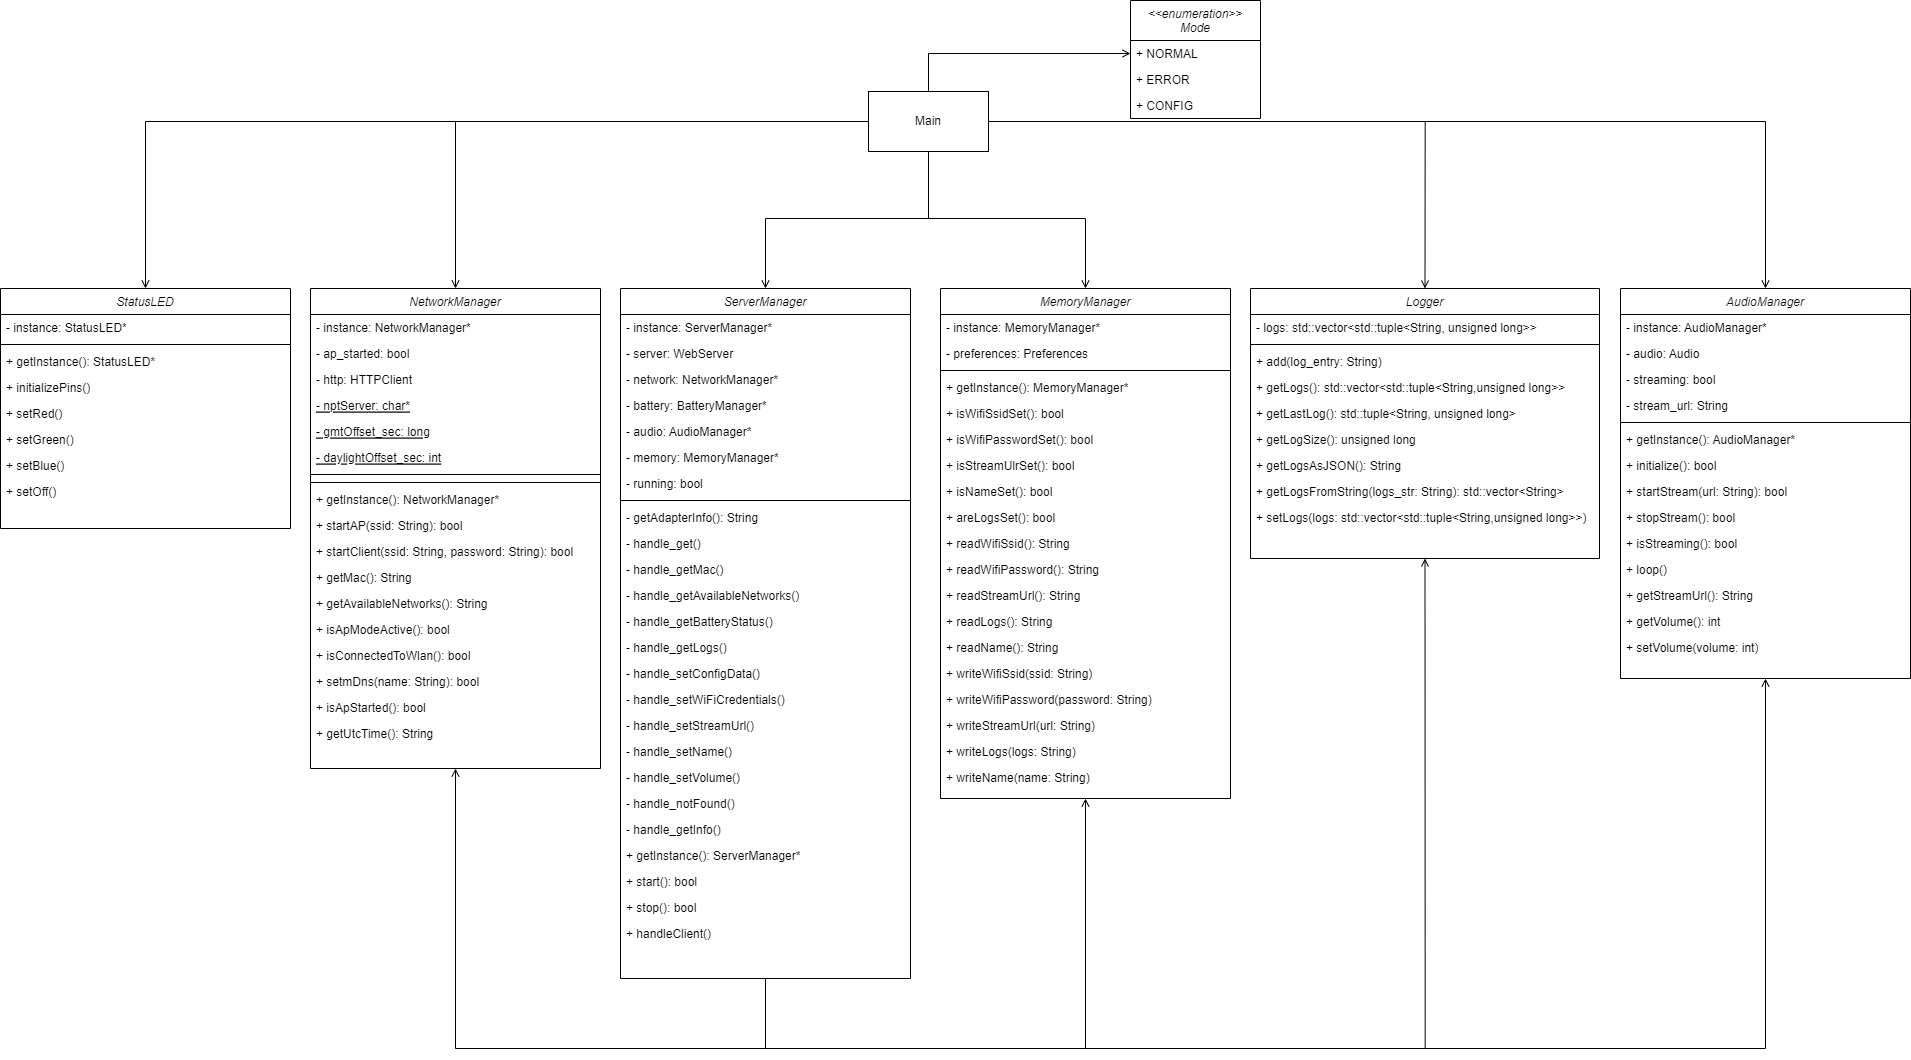
\includegraphics[width=0.9\textheight, angle=90]{/software/uml_microcontroller.png}
	\caption{UML-Klassendiagramm Mikrocontroller}
\end{figure}
\noindent
Im Folgenden werden die einzelnen Klassen genauer beschrieben: \\
\textbf{Mode} \newline
Im ENUM \glqq Mode\grqq{} werden die verschiedenen Modi der Software definiert. Ein ENUM ist wie eine Art Datentyp, der Konstanten definiert, welche man verwenden darf. \parencite[vgl.][]{noauthor_urlpi15_nodate} In unserem Fall definiert der ENUM die drei Modi \glqq NORMAL\grqq{}, \glqq CONFIG\grqq{} und \glqq ERROR\grqq{}. Diese geben den Status des MAA an. Der Modus \glqq NORMAL\grqq{} signalisiert, dass sich der MAA im normalen Zustand befindet, dieser also voll funktionsfähig ist. Im Modus \glqq CONFIG\grqq{} fungiert der MAA als Access Point. Somit können sich Clients mit diesem verbinden und die Anmeldedaten des WLANs senden. Der Modus \glqq ERROR\grqq{} wird gesetzt, wenn ein Fehler im Programm auftritt. Dies ist zum Beispiel der Fall, wenn die Verbindung mit dem WLAN unterbrochen wird. Der aktuelle Modus wird mithilfe der Status-LED signalisiert, welche als nächstes genauer beschrieben wird. \newline \\
\textbf{StatusLED} \\
Mithilfe der Klasse \glqq StatusLED\grqq{} wird die RGB-LED, welche am Mikrocontroller angeschlossen ist, gesteuert. Mit ihr wird der aktuelle Modus des MAA dem/der Benutzer/in angezeigt. Die nachstehende Tabelle beschreibt, welche Farbe für welchen Modus steht: \newline \\
\begin{table}[H]
	\begin{tabular}{|l|l|}
		\hline
		\textbf{Modus} & \textbf{Farbe} \\
		\hline
		NORMAL & Grün \\
		\hline
		CONFIG & Blau \\
		\hline
		ERROR & Rot \\
		\hline
	\end{tabular}
	\caption{Status-Farben}
\end{table}
\noindent %dass Text nach figure nicht eingerückt wird
\textbf{NetworkManager}\newline
Die Klasse \glqq NetworkManager\grqq{} beinhaltet Funktionen, welche die Wi-Fi-Funktionalität des ESP32 verwenden. Es ist hier möglich, den Access Point - und den Client-Modus zu aktivieren, nach verfügbaren Netzwerken zu suchen, sowie die MAC-Adresse des Adapters zu lesen. Diese Funktionen werden alle mithilfe der im Kapitel 3.6.2 erwähnten \glqq WiFi\grqq{}-Bibliothek verwirklicht.
\vspace{4mm}\newline
\textbf{AudioManager}\newline
Die Klasse \glqq AudioManager\grqq{} ist für den Empfang des Internetradio-Streams, für das Dekodieren des empfangenen Streams und für die Ausgabe des dekodierten Audio-Signals zuständig. Dafür wird primär die \glqq ESP8266Audio\grqq{}-Bibliothek, welche bereits im Kapitel 3.6.2 beschrieben wurde, verwendet.
\vspace{4mm}\newline
\textbf{Logger}\newline
Die Klasse \glqq Logger\grqq{} ist für die Verwaltung von Logs, welche von anderen Klassen geschrieben werden, zuständig. In ihr befindet sich ein Vektor, welcher Tupels, bestehend aus Log-Text und Log-Zeitpunkt, speichert, definiert. Diese Logs sind essenziell für die Fehlerbehebung, da man sehen kann, welche Aktionen im Programm ausgeführt wurden und wo Fehler aufgetreten sind. Die Klasse bietet Funktionen zum Hinzufügen von Logs und zum Anzeigen bestehender Logs. Die Funktionen sind alle statisch, das heißt, man muss kein Objekt dieser Klasse erzeugen, um die Funktionen auszuführen. Dies ist sinnvoll, weil es möglich sein soll, von jeder Klasse direkt auf die Log-Funktionen zuzugreifen.
\vspace{4mm}\newline
\textbf{ServerManager}\newline
Die Klasse \glqq ServerManager\grqq{} ist für das Verwalten des Webservers, welcher auf dem MAA läuft, zuständig. In ihr werden die Funktionen, die durch die Aufrufe der Routen der REST-API ausgeführt werden, definiert. Die Kernfunktionen der Klasse werden vor allem durch die im Kapitel 3.6.2 erwähnte \glqq WebServer\grqq{}-Bibliothek bereitgestellt.
\vspace{4mm}\newline
\textbf{MemoryManager} \newline
Die Klasse \glqq MemoryManager\grqq{} ist für das Schreiben in und das Lesen aus dem EEPROM des Mikrocontrollers zuständig. Der EEPROM ist ein nichtflüchtiger Speicher, das heißt, er behält die Daten auch nach einem Spannungsverlust des Mikrocontrollers. Dies ist vor allem für Daten sinnvoll, welche nicht jedes Mal neu definiert werden, wie z.B. Anmeldedaten des WLANs. \parencite[vgl.][]{santos_urlpi27_2018}
Um die Funktionen des EEPROMs des ESP32 zu nutzen, wurde die \glqq Preferences\grqq{}-Bibliothek, welche ebenfalls im Kapitel 3.6.2 beschrieben wurde, verwendet. Diese arbeitet mit Schlüssel-Wert-Paaren. Das heißt, auf die gespeicherten Variablen kann mittels eindeutigem Schlüssel zugegriffen werden.
\newline \\
\textbf{BatteryManager} \newline
Die Klasse \glqq BatteryManager\grqq{} ist für das Auslesen des Akkustands des ESP32 zuständig. Dies wird erreicht, indem der Spannungspegel an einem analogen Eingang des ESP32 eingelesen wird und aus diesem dann der Ladestand des Akkus errechnet wird.
\subsubsection{Programmablauf}
Da die \glqq Arduino-Core\grqq{}-Bibliothek verwendet wurde, ist der Programmablauf gleich wie bei einem standardmäßigen Arduino-Programm. Ausgeführt wird die Main-Datei, welche aus den Funktionen \glqq setup\grqq{} und \glqq loop\grqq{} besteht. Die Setup-Funktion wird beim Start des Mikrocontrollers einmalig ausgeführt. In ihr werden also alle Funktionen, die für den weiteren Verlauf des Programms essenziell sind, ausgeführt. Anschließend wird die Loop-Funktion in einer Endlosschleife ausgeführt. Wenn also das Ende der Loop-Funktion erreicht wird, fängt diese wieder von vorne an. Im folgenden Teil wird der Ablauf innerhalb der einzelnen Funktionen genauer beschrieben.
\vspace{4mm}\newline
\textbf{Setup} \newline
Im folgenden UML-Ablaufdiagramm wird der grobe Programmablauf der Setup-Funktion dargestellt:
\begin{figure}[H]
	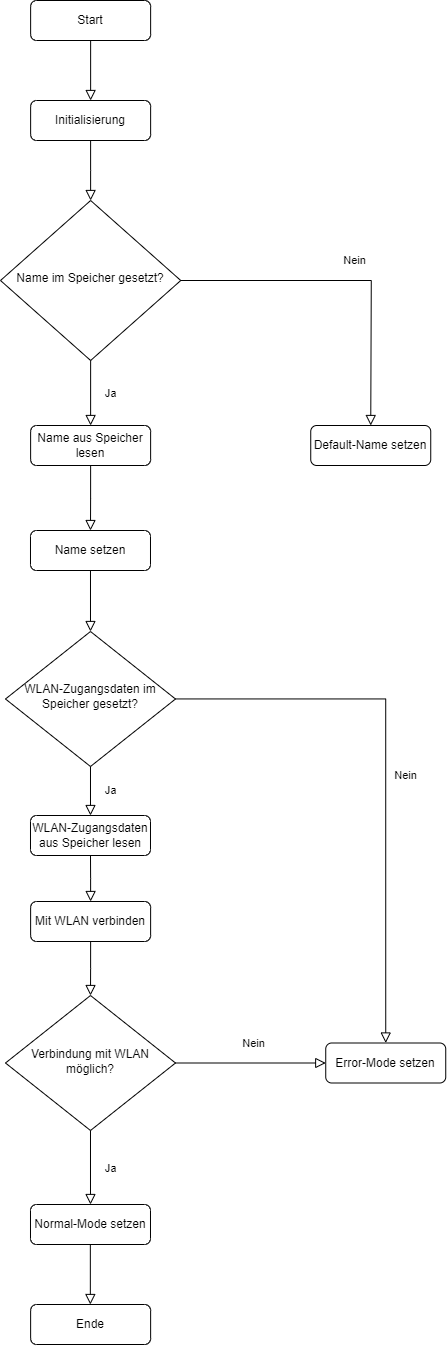
\includegraphics[height=0.95\textheight]{/software/uml_ablauf_esp32_setup.png}
\caption{UML-Ablaufdiagramm Mikrocontroller Setup}
\end{figure}
In der Setup-Funktion werden zuerst Konstanten, welche später im Programm benötigt werden, definiert. Auch werden am Anfang die entsprechenden Instanzen der Singleton-Klassen abgerufen. Anschließend wird der Name des Adapters definiert. Dieser setzt sich, wie bereits im Kapitel 3.5.1 erwähnt, aus \glqq MAA\grqq{} und den letzten drei Byte der MAC-Adresse zusammen. Er ist somit für jeden Adapter eindeutig. Der Name wird später als SSID des Access Points bzw. als Hostname für den Webserver verwendet. Nachdem der Name gesetzt ist, wird mit der Klasse \glqq MemoryManager\grqq{} abgefragt, ob WLAN-Anmeldedaten im EEPROM gespeichert sind. Sind diese vorhanden, so versucht der MAA eine Verbindung mit dem WLAN herzustellen. Ist dies möglich, wird der Modus auf \glqq NORMAL\grqq{} gesetzt. Schlägt die Verbindung mit dem WLAN, z.B. durch falsche Anmeldedaten, fehl, wird der Modus auf \glqq ERROR\grqq{} gesetzt. \newline \\
\textbf{Loop} \newline
Im folgenden UML-Ablaufdiagramm wird der grobe Programmablauf der Loop-Funktion dargestellt:
\begin{figure}[H]
	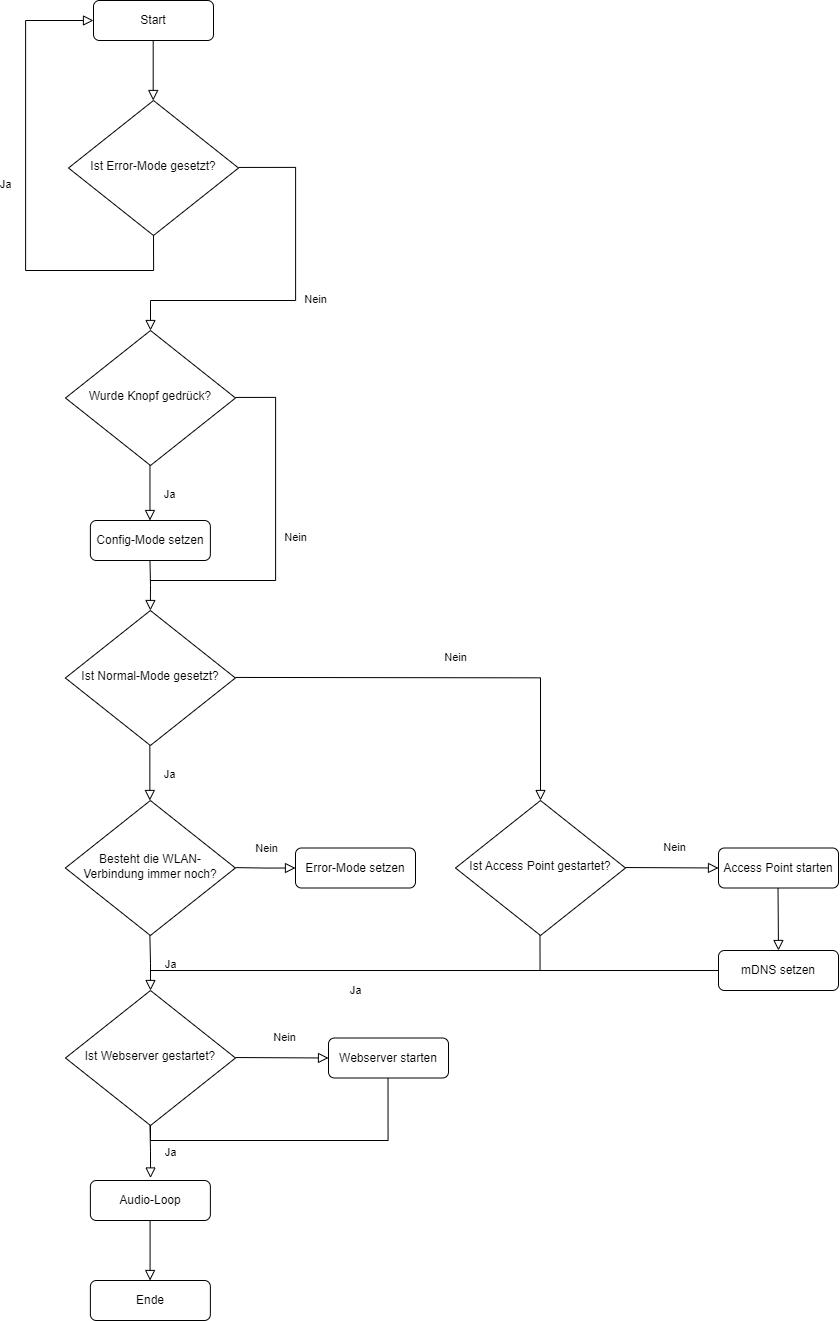
\includegraphics[height=0.95\textheight]{/software/uml_ablauf_esp32_loop.png}
	\caption{UML-Ablaufdiagramm Mikrocontroller Loop}
\end{figure}
Am Anfang der Loop-Funktion wird abgefragt, ob der Modus auf \glqq ERROR\grqq{} gesetzt ist. Ist dies der Fall, wird nichts mehr ausgeführt, das heißt, die Funktion springt wieder an den Startpunkt. Ist der Modus allerdings nicht auf \glqq ERROR\grqq{} gesetzt, wird überprüft, ob der Knopf gedrückt ist. Ist dieser gedrückt, wird der Modus auf \glqq CONFIG\grqq{} gesetzt. Anschließend wird überprüft, ob der Modus auf \glqq NORMAL\grqq{} gesetzt ist. Ist dies der Fall, wird überprüft, ob immer noch eine Verbindung mit dem WLAN besteht. Dies geschieht mithilfe der Klasse \glqq NetworkManager\grqq{}. Wenn eine WLAN-Verbindung besteht, wird mithilfe der Klasse \glqq ServerManager\grqq{} überprüft, ob der Webserver läuft. Wenn nicht, wird dieser gestartet. Ist der Modus allerdings nicht auf \glqq NORMAL\grqq{} gesetzt, also auf \glqq CONFIG\grqq{}, so wird zuerst überprüft, ob der Access Point - Modus gestartet ist, da dieser für die Verbindung zwischen Client (Smartphone) und Server (MAA) benötigt wird. Wenn nicht, wird dieser schließlich gestartet und das mDNS-Protokoll, welches bereits im Kapitel 3.5.1 beschrieben wurde, wird konfiguriert. Diese Prozesse werden wieder mithilfe der \glqq NetworkManager\grqq{}-Klasse durchgeführt. Anschließend wird ebenfalls der Zustand des Webservers überprüft. Am Schluss der Loop-Funktion wird noch die Loop-Funktion der Klasse Audio-Manager ausgeführt. Diese regelt das Audiostreaming.
\subsubsection{Erweiterungsmöglichkeiten}
In Zukunft sind noch weitere Funktionalitäten, welche außerhalb der Diplomarbeit implementiert werden, für die Software geplant. Im Hinblick auf die Sicherheit wäre es durchaus sinnvoll, den Webserver des Mikrocontrollers auf HTTPS umzustellen. Somit wäre eine verschlüsselte Kommunikation mit diesem möglich. Zusätzlich wäre es auch denkbar eine Funktion zu implementieren, die es ermöglicht mehrere Adapter zu Gruppen zu verbinden. In diesen Gruppen soll dann jeweils der gleiche Audiostream synchron empfangen und ausgegeben werden. Die Synchronisierung der Adapter bringt aber eine hohe Komplexität mit sich, da man per WLAN-Verbindung mit sehr großen Latenzen zu rechnen hat. Ein Ansatz wäre zum Beispiel, dass jeder Mikrocontroller in einem bestimmten Intervall die Zeit von einem NTP (Network Time Protocol) - Server abfragt und somit auf allen Mikrocontrollern die Zeit annähernd gleich ist. Dann könnte man die Buffer, welche vom Audiostream erhalten werden, mit einem Zeitstempel versehen und sie beim Erreichen dieser Zeit abspielen. Das Hauptproblem dieser Lösung wäre, dass die Zeitdifferenz zwischen den Mikrocontrollern vermutlich zu groß wäre und somit eine hörbare Latenz entsteht.
\subsection{Entwicklung Smartphone-App}
In diesem Kapitel wird der Übergang der Planung in die Entwicklung der Smartphone-App beschrieben.
\subsubsection{Struktur}
In diesem Kapitel wird der Aufbau bzw. die Struktur der Smartphone-App genauer beschrieben. Die folgende Grafik stellt dabei die grobe Struktur der App dar:
\begin{figure}
	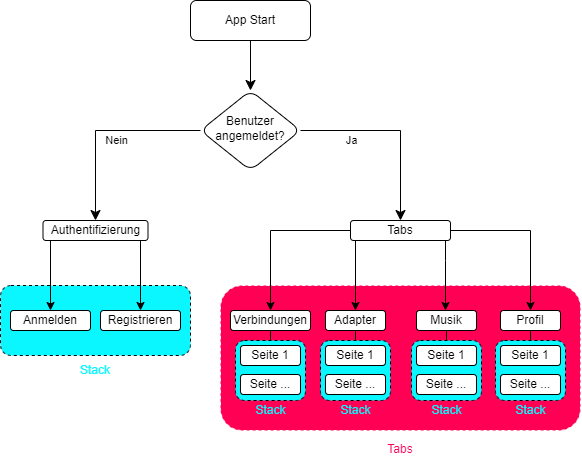
\includegraphics[width=\textwidth]{/software/app_struktur.png}
\caption{Struktur Smartphone-App}
\end{figure}
\FloatBarrier
\textbf{Navigation} \newline
Für die Navigation zwischen den Seiten der App wurde einerseits die Tab-Navigation und andererseits die Stack-Navigation von \glqq Expo Router\grqq{} verwendet. Dabei wird grob zwischen dem Ordner \glqq auth\grqq{} und dem Ordner \glqq tabs\grqq{} unterschieden. Der Ordner \glqq auth\grqq{} enthält die Seiten, welche für die Benutzerauthentifizierung, also Login und Registrierung, notwendig sind. Der Ordner \glqq tabs\grqq{} hingegen enthält alle Seiten, welche für registrierte Benutzer sichtbar sind und somit die eigentliche App darstellen. Die App ist grundlegend in die vier Tabs \glqq Verbindungen\grqq{}, \glqq Adapter\grqq{}, \glqq Musik\grqq{} und \glqq Profil\grqq{}  gegliedert. Zwischen diesen Tabs kann mithilfe der Tab-Bar, welche unten in der App sichtbar ist, gewechselt werden. In den einzelnen Tabs befinden sich jeweils mehrere Seiten. Zwischen diesen Seite kann mittels Stack-Navigator gewechselt werden. Der Stack-Navigator arbeitet dabei nach dem sogenannten \glqq Last In - First Out\grqq{}- Prinzip (LIFO). Das heißt, dass die Seite, welche als letztes zum Stack (Stapel) hinzugefügt wurde, als Erstes wieder von diesem entfernt wird. Somit wird die Navigations-Historie festgehalten und der/die Benutzer/in kann jederzeit wieder auf die vorherigen Seiten zurückgehen. \parencite[vgl.][]{noauthor_urlpi28_nodate}
\subsubsection{Design}
Beim Style des User Interface der App wurde auf Übersichtlichkeit und wenig Komplexität gesetzt. Der/Die Benutzer/in soll sich in der App schnellstmöglich zurechtfinden. Durch die gute Benutzbarkeit werden allerdings gleichzeitig die Konfigurationsmöglichkeiten eingeschränkt, was die Flexibilität der App senkt. Bei der Auswahl der Farben, welche in der App sichtbar sind, wurde darauf geachtet, dass diese die App modern und schlicht erscheinen lassen. Für die App wurde ein Darkmode implementiert, weil dieser in den meisten modernen Applikationen verwendet wird und dieser die App somit moderner aussehen lässt.
\textbf{Farben} \\
Bei der Farbauswahl wurden als Hauptfarben eher dunklere Farben verwendet, um die App im Darkmode darzustellen. Im Kontrast zu den primär dunklen Farben wurden knallige, satte Farben im Torquise-Ton für die Steuerelemente, wie z.B. Buttons verwendet. Im Folgenden ist eine Tabelle mit den verwendeten Farben und deren Farbcodes im Hex-Format abgebildet: \\
\begin{table}
	\begin{tabular}{|l|l|l|}
        \hline
        \textbf{Bezeichnung} & \textbf{Farbcode (hex)} & \textbf{Farbe} \\ 
        \hline
        grey & \#2B2C28 & \fcolorbox{black}{grey}{\phantom{XX}} \\ 
        \hline 
        lightTurquoise & \#7DE2D1 & \fcolorbox{black}{lightTurquoise}{\phantom{XX}} \\ 
        \hline 
        white & \#FFFAFB & \fcolorbox{black}{whiteColor}{\phantom{XX}} \\ 
        \hline 
        red & \#D90B0B & \fcolorbox{black}{redColor}{\phantom{XX}} \\ 
        \hline 
        lightGrey & \#3E403A & \fcolorbox{black}{lightGrey}{\phantom{XX}} \\ 
        \hline 
    \end{tabular} 
	\caption{App-Farben}
\end{table}
\FloatBarrier
\subsubsection{Komponenten}
Wie bereits im Kapitel 3.4.3 erwähnt, bietet React Native die Möglichkeit eigene Komponenten zu erstellen. Als Grundlage dafür dienen die Standardkomponenten von React Native. Der Vorteil bei der Verwendung von Komponenten ist, dass diese wiederverwendbar sind und ein bestimmtes Verhalten aufweisen. Man muss also den Code für eine Komponente nur einmal schreiben und kann diese Komponente dann in der gesamten App verwenden. Im Folgenden werden die wichtigsten Komponenten, welche selbst erstellt wurden, aufgezählt und kurz beschrieben. \newline \\
\begin{itemize}
	\item \textbf{AdapterItem} 
	\par Zeigt die Daten eines Adapters an. Wenn dieser nicht verbunden ist, wird dies mit einem grauen Hintergrund und einem Symbol einer durchgestrichenen Wolke signalisiert.
	\begin{flushleft}
    		\captionsetup{type=figure}
     	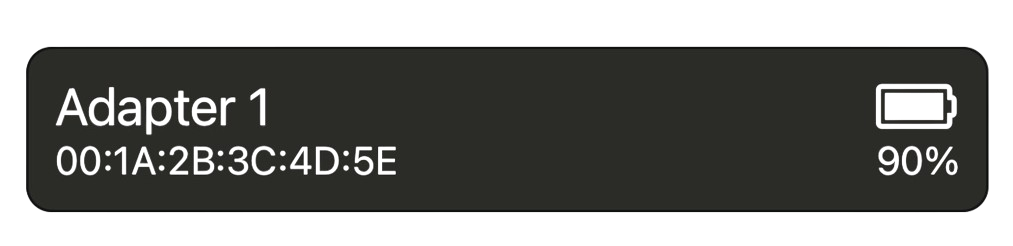
\includegraphics[width=0.4\textwidth]{/software/adapter_item.png}
    		\caption{AdapterItem-Komponente}
    	\end{flushleft}
	\item \textbf{StationItem}
	\par Zeigt die Daten einer Internetradiostation an.
	\begin{flushleft}
    		\captionsetup{type=figure}
     	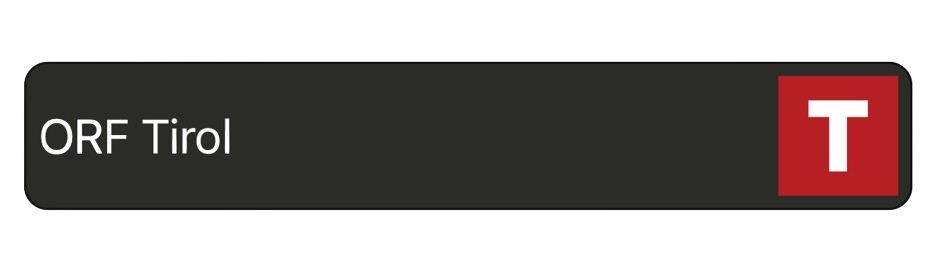
\includegraphics[width=0.4\textwidth]{/software/station_item.png}
    		\caption{StationItem-Komponente}
    	\end{flushleft}
	\item \textbf{ConnectionItem}
	\par Stellt eine Verbindung zwischen Radiostation und Adapter dar. Dabei werden die StationItem-Komponente und die AdapterItem-Komponente verwendet. Die Komponente ermöglicht es auch, den aktuellen Stream des Adapters zu stoppen bzw. die Lautstärke des Streams zu regeln.
	\begin{flushleft}
    		\captionsetup{type=figure}
     	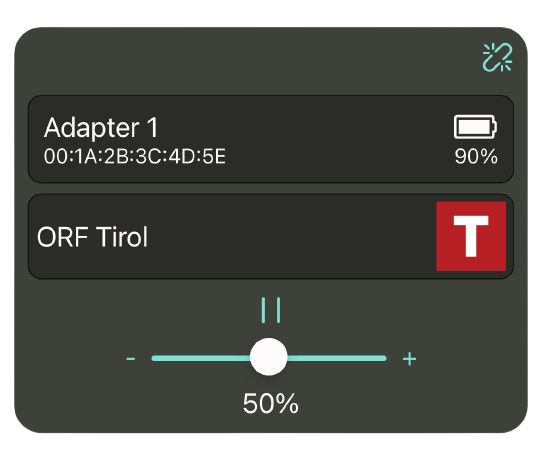
\includegraphics[width=0.4\textwidth]{/software/connection_item.png}
    		\caption{FavouriteStationList-Komponente}
    	\end{flushleft}
	\item \textbf{AdapterList}
	\par Erstellt eine Liste aus mehreren AdapterItem-Komponenten. Realisiert außerdem die Möglichkeit, einen Adapter zu löschen.
	\item \textbf{FavouriteStationList}
	\par Erstellt eine Liste, in der alle Stationen, welche sich in der Favoritenliste des Benutzers befinden, mithilfe von StationItem-Komponenten dar.
	\begin{flushleft}
    		\captionsetup{type=figure}
     	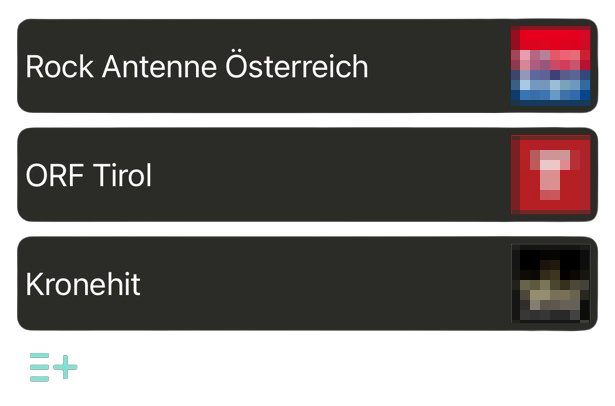
\includegraphics[width=0.4\textwidth]{/software/station_list.png}
    		\caption{FavouriteStationList-Komponente}
    	\end{flushleft}
	\item \textbf{Connectionlist}
	\par Erstellt eine Liste, in der sich die aktuellen Verbindungen zwischen Adaptern und Radiostationen, dargestellt durch ConnectionItem-Komponenten, dar. Die Komponente ermöglicht es zudem Verbindungen zu trennen.
	\begin{flushleft}
    		\captionsetup{type=figure}
     	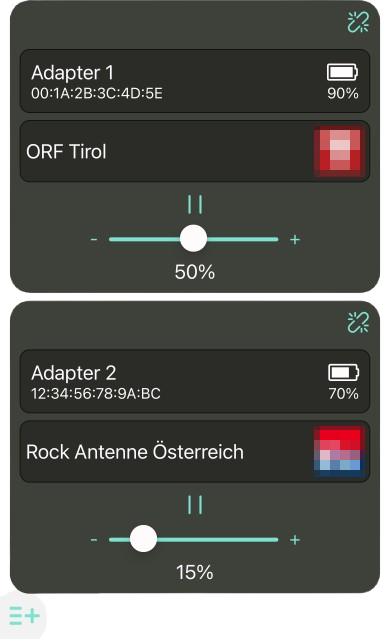
\includegraphics[width=0.4\textwidth]{/software/connection_list.png}
    		\caption{FavouriteStationList-Komponente}
    	\end{flushleft}
	\item \textbf{ErrorScreen}
	\par Stellt eine Ansicht bereit, die signalisiert, dass irgendwo ein Fehler aufgetreten ist. Als Parameter wird dieser Komponente der Fehlertext und die Aktion, welche der/die Benutzer/in als Reaktion auf den Fehler ausführen kann, mitgegeben.
	\item \textbf{LoadingScreen}
	\par Stellt eine Lade-Animation dar und einen Text, der als Parameter übergeben wird. Diese Ansicht soll signalisieren, dass Daten in der App geladen werden und der/die Benutzer/in deshalb warten muss.
\end{itemize}
\subsubsection{Seiten}
Wie bereits im Kapitel Struktur erwähnt, besteht die App aus mehreren Seiten, zwischen diesen mit verschiedenen Navigationsarten gewechselt werden kann. Eine Seite setzt sich dabei aus den Grundkomponenten von React Native und den selbst erstellten Komponenten, welche im Kapitel Komponenten genauer beschrieben wurden, zusammen. Dabei ist die Grundstruktur jeder Seite gleich. Wie man in Abbildung ... sehen kann, befindet sich oben ein Header, der den Namen der aktuellen Seite anzeigt, und unten die Tab-Bar welche anzeigt, in welchem Tab man sich aktuell befindet.
Im Folgenden werden die einzelnen Seiten der App aufgezählt und kurz beschrieben.
\begin{itemize}
	\item \textbf{Anmelden} 
	\par Ermöglicht es einem Benutzer / einer Benutzerin, sich in der App anzumelden.
	\item \textbf{Registrieren} 
	\par Ermöglicht es einem Benutzer / einer Benutzerin, sich neu zu registrieren.
	\item \textbf{Startseite Verbindungen} 
	\par Zeigt die aktuellen Verbindungen mithilfe der ConnectionList-Komponente an. Auf dieser Seite ist es möglich, bestehende Verbindungen zu verwalten und zu trennen.
	\item \textbf{Verbindung hinzufügen}
	\par Ermöglicht es, eine neue Verbindung zwischen einem Adapter und einer Internetradiostation anzulegen.
	\item \textbf{Startseite Adapter}
	\par Zeigt alle gespeicherten Adapter des Benutzers / der Benutzerin an. Hier ist es außerdem möglich, Adapter zu löschen.
	\item \textbf{Adapter hinzufügen}
	\par Ermöglicht es, einen neuen Adapter hinzuzufügen bzw. diesen zu konfigurieren.
	\item \textbf{Stationen filtern}
	\par Ermöglicht es, das Land bzw. die Sprache auszuwählen, nach denen dann in weiterer Folge die Stationen, welche auf der Seite \glqq Stationen auswählen\grqq{} angezeigt werden.
	\item \textbf{Stationen auswählen}
	\par Ermöglicht es, mehrere Stationen auszuwählen, welche dann in die Favoritenliste des Benutzers / der Benutzerin übernommen werden. Es werden nur Stationen angezeigt, die den Filteroptionen, welche auf der Seite \glqq Stationen filtern\grqq{} festgelegt wurden, angezeigt.
	\item \textbf{Profil}
	\par Hier werden Informationen zum Profil des Benutzers / der Benutzerin angezeigt. Auf dieser Seite wird dem/der Benutzer/in außerdem ermöglicht sich abzumelden bzw. sein/ihr Passwort zurückzusetzen.
\end{itemize}
\subsubsection{APIs}
In diesem Kapitel werden die APIs (Application Programming Interfaces) beschrieben, mit welchen die App Daten austauscht. \newline \\
\textbf{RadioBrowser-API}\\
Die RadioBrowser-API ist eine open-source API welche eine sehr umfangreiche Sammlung von Internet-Radios bereitstellt. Dabei ist es einerseits möglich, mithilfe dieser API neue Radiostationen zu der Sammlung hinzuzufügen und andererseits, bestehenden Radiostationen nach bestimmten Suchkriterien zu suchen und die Daten derer abzufragen. \parencite[vgl.][]{noauthor_urlpi21_nodate} In der Smartphone-App wird die RadioBrowser-API verwendet, um nach Radiosendern zu suchen und in weiterer Folge die Stream-URLs dieser an den MAA zu senden. Der MAA ruft in weiterer Folge den jeweiligen Audiostream auf und empfängt diesen. \newline \\
\textbf{Firebase}\\
Firebase ist eine Entwicklungsplattform von Google, welche verschiedene Dienste, die hilfreich für die Entwicklung von Apps bzw. Web-Apps sind, bereitstellt. Firebase stellt dabei ein Backend für die Apps dar. Damit werden Prozesse, wie z.B. Benutzerauthentifizierung, Speicherung von Benutzern und Speicherung von Daten nicht lokal auf dem Gerät, sondern in der Cloud ausgeführt \parencite[vgl.][]{noauthor_urlpi22_nodate} In der Smartphone-App wurde Firebase zur Benutzerverwaltung verwendet. Dabei wurde einerseits der \glqq Firebase Authentication\grqq{}-Dienst für die Benutzerauthentifizierung und andererseits der \glqq Cloud Firestore\grqq{}-Dienst für die Speicherung von Benutzerdaten verwendet. Firebase wurde für die Entwicklung der Smartphone-App gewählt, da dadurch der Ressourcenverbrauch der App minimiert wird und der/die Benutzer/in von jedem Gerät aus Zugriff auf seine/ihre Daten hat und somit nicht auf ein bestimmtes Gerät angewiesen ist. Außerdem müssen Dienste, wie z.B. die Benutzerauthentifizierung nicht neu entwickelt werden.
\subsubsection{Zustandsverwaltung}
Um Zustände, welche in mehreren Teilen der App benötigt werden, global bereitzustellen, wurde die Context-Funktionalität von React Native verwendet. Context ermöglicht es Zustände global in der App bereitzustellen und diese in den einzelnen Komponenten aufzurufen. Dabei werden bei der Änderung eines Zustands die betroffenen Komponenten sofort aktualisiert. Um den Context bereitzustellen, wird ein sogenannter Context-Provider verwendet. Alle Komponenten welche in den Context-Provider eingebettet sind, können auf den Zustand von diesem zugreifen. \parencite[vgl.][]{noauthor_urlpi23_nodate} In der Smartphone-App wurden folgende ContextProvider definiert:
\begin{itemize}
	\item \textbf{UserContext}
	\par Stellt das Benutzerobjekt bereit. Dieses beinhaltet wichtige Benutzerdaten, welche an mehreren Stellen der App verwendet werden. Das Benutzerobjekt wird von Firebase Authentication abgefragt.
	\item \textbf{AdapterContext}
	\par Stellt eine Liste von hinzugefügten Adaptern bereit. Diese Liste wird von Firebase Firestore abgefragt. Falls sich die in Firestore gespeicherte Liste ändert, wird die Liste, welche der AdapterContext bereitstellt, automatisch aktualisiert. 
	\item \textbf{StationContext}
	\par Stellt eine Liste von hinzugefügten Radiostationen bereit. Diese Liste wird ebenfalls von Firebase Firestore abgefragt. Die hier gespeicherte Liste wird ebenfalls automatisch aktualisiert, falls sich die Liste in Firestore ändert.
\end{itemize}
\subsubsection{Benutzerverwaltung}
Die Benutzerdaten sind durch ein im UserContext gespeichertes Benutzerobjekt in der gesamten App global verfügbar. Das Objekt wird am Anfang der App, falls vorhanden, aus dem lokalen Gerätespeicher ausgelesen oder mittels Login von Firebase abgefragt. Der Status des Benutzerobjektes wird mittels eines Event-Handlers verfolgt. Das heißt, wenn sich der Status des Benutzerobjektes, z.B. durch einen Logout, ändert, wird 
Die Verwaltung von Benutzerdaten wurde primär mit Firebase (siehe APIs) verwirklicht. Beim Start der App wird abgefragt ob im lokalen Speicher ein Benutzer-Objekt gespeichert ist. Wenn dies der Fall ist, ist der Teil Tabs für den/die Benutzer/in erreichbar. Ist dies nicht der Fall, so wird der/die Benutzer/in zur Login-Seite weitergeleitet. Dort ist es möglich 
\subsubsection{Erweiterungsmöglichkeiten}
In Zukunft wäre es noch denkbar, außerhalb der Diplomarbeit weitere Funktionen in die Smartphone-App zu implementieren. Dabei wäre es durchaus sinnvoll mehrere Audio-Streaming-Quellen, wie zum Beispiel Musikstreamingdienste (Spotify, Amazon Music etc.) einzubinden. Außerdem könnte man das Erstellen von Adapter-Gruppen realisieren, sodass mehrere Adapter zu einer Gruppe zusammengefügt werden können und diese dann den gleichen Stream ausgeben. Um dies umzusetzen, müsste allerdings auch die Software des Adapters weiterentwickelt werden.
\subsection{Design Adaptergehäuse}
Das Adaptergehäuse trägt einen wesentlichen Teil zur Sicherheit des Endverbrauchers sowie zur optimalen
Funktionalität der Komponenten bei. Zudem soll es möglichst kompakt sein.
\subsubsection{Grundsätzlicher Aufbau}
Die Grundlage für den Prototyp bildet ein Kasten mit Deckel.\newline
Das Gehäuse wurde mit frei schwebenden, jedoch an den Wänden befestigten Stützen ausgestattet, um den Mikrocontroller fest montieren zu können. Der Prototyp wurde zudem mit kleinen Zylindern auf den Stützen ausgestattet, um den Mikrocontroller mit seinen bereits Vorhandenen Aussparungen darauf platzieren zu können. Der Digital-/Analogwandler und der Akku-Laderegler finden auch auf solchen Stützen ihren Platz. Der Gedanke dahinter war, den Akku unter den Bauteilen zu platzieren. Mehr dazu im Teil "Wärmeableitung". Zudem wurden in einer Wand des Gehäuses Aussparungen für die Buchsen platziert. Die Aussparungen für die RGB-LED und den Taster wurden im Deckel platziert. Eine Art Abdeckung für den Taster selbst wird auf diesen geklebt um ein gleichbleibendes Erscheinungsbild des Gehäuses zu behalten. Der Deckel, der von oben auf das Gehäuse gedrückt wird, schließt dieses. Im Deckel ist zusätzlich ein Belüftungsgitter eingelassen.
\subsubsection{Wärmeableitung}
Wärmeableitung ist wichtig, da Mikrocontroller, wie alle anderen Prozessoren auch, bei intensivem Betrieb Hitze entwickeln. Laut einer eigens durchgeführten Messung wird der in diesem Fall eingesetzte ESP32 meistens nur rund 38°C warm. Bei hoher Rechenleistung sind jedoch auch höhere Temperaturen möglich. Der ESP32 hat laut Hersteller eine mögliche Betriebstemperatur (Umgebungstemperatur) von –40°C bis +125°C. Damit die entstandene Wärme gut ableiten kann und keine der Komponenten stark beeinflusst (vor allem den Akku, da dieser bei hohen Temperaturen eine Explosionsgefahr darstellt), wird der Mikrocontroller im Gehäuse oben, also auf Stützen angebracht. Die aufsteigende Wärme kann somit nach oben durch das dafür vorgesehene Gitter entweichen und staut sich somit nicht im Inneren des Gehäuses. Der Akku liegt dementsprechend unter dem Mikrocontroller und allen anderen Komponenten und wird durch die abstrahlende Hitze dementsprechend nur etwas wärmer als Raumtemperatur.
\vspace{4mm}\newline
\parencite[vgl.][]{noauthor_urlnl06_nodate}
\subsubsection{Virtuelles 3D-Design}
Um ein 3D-Modell des Prototypen zu zeichnen, wurde AUTODESK Fusion verwendet. Der Anbieter beschreibt seine Software folgendermaßen: "Autodesk Fusion verbindet Ihren gesamten Fertigungsprozess durch die Integration von CAD, CAM, CAE und PCB in einer einzigen Lösung, mit der Sie Ihre Ideen verwirklichen und praktisch alles fertigen können."\newline
Wenn man schon früh beachtet, dass die Prototypen mit einem 3D-Drucker gefertigt werden, kann man schon das 3D-Design für eine gute Druckbarkeit auf 3D-Drucker anpassen. Damit ist hauptsächlich gemeint, überhängende Drucke, komplizierte Stützstrukturen oder ähnliches zu vermeiden.
\vspace{4mm}\newline
\textbf{Basis} \newline
Die Basis des Adapters bildet ein 71x58x27mm großer Kasten mit 2mm Wanddicke. Aus Erfahrung kann man sagen, dass diese Dicke bei 3D-Drucken stabil ist, während sie jedoch nicht zu klobig wirkt.\newline
Die Stützen des Mikrocontroller beginnen auf 11mm Höhe und sind auf einer Längenseite 6x6x5mm und auf der anderen 6,9x6x5mm groß. Sie sind jeweils mit einer oder zwei Seiten an der Wand der Basis und somit überhängend. Dies wird im Teil "Drucken des Prototyps/Stützstruktur" noch wichtig.\newline
\begin{figure}[H]
\begin{flushleft}
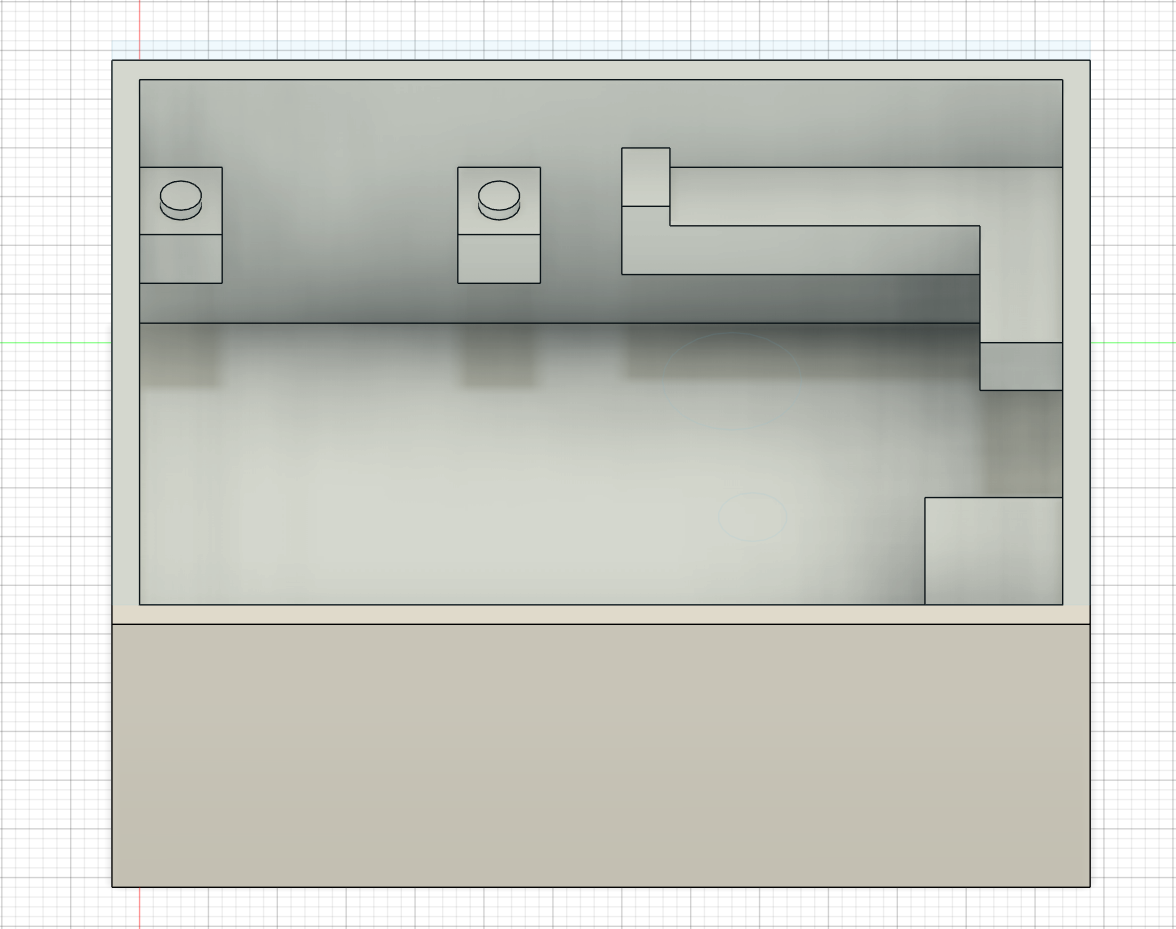
\includegraphics[scale=0.5]{/hardware/stuetzen_fusion.png}
\caption{Abbildung der Stützen für die Komponenten}
\end{flushleft}
\end{figure}
Auf den Stützen befinden sich jeweils Zylinder, die genau auf die Aussparungen des Mikrocontroller vermessen wurden. Die Zylinder haben einen Durchmesser von exakt 3mm. Der Abstand der Mittelpunkte dieser Zylinder war bei unserem Modell 47,10mm in der Länge und 23,10mm in der Breite. Auf einer Seite befindet sich zwischen Wand und Zylinder etwas mehr Platz, da der USB-C Port des Mikrocontrollers etwas über diesen herausragt. Deswegen auch der zuletzt erwähnte Versatz der Stütze von 0,9mm.\newline
Die Breite der Basis ist also genau auf die Länge von dem von uns benutzten Mikrocontroller zugeschnitten.\newline
In den gegenüberliegenden Ecken der Basis befinden sich der Digital-/Analogwandler und der Laderegler. Die Maße des Digital-/Analogwandler sind 31,8x17,2mm. Die Maße des Laderegler sind 28x17,45mm. Beide liegen, wie der Mikrocontroller auch, auf überhängenden, 5mm hohen Stützen auf. Aufgrund der USB-C Buchse wird der Halt des Laderegler noch von einer 3,5mm breiten 2mm-Erhöhung am Ende der Stütze verstärkt. Die USB-C Buchse wurde passend zum Laderegler und der Norm entsprechend (8,34x2,56mm Größe) eingelassen. Der Digital-/Analogwandler wird aufgrund der 3,5mm Klinkenbuchse von einer herabstehenden Wand gestützt, die im Teil "Deckel" genauer beschrieben wird. Die Aussparung der AUX-Buchse wurde auch passend für den Digital-/Analogwandler platziert und hat einen Durchmesser von 6mm.\newline
\begin{figure}[H]
\begin{flushleft}
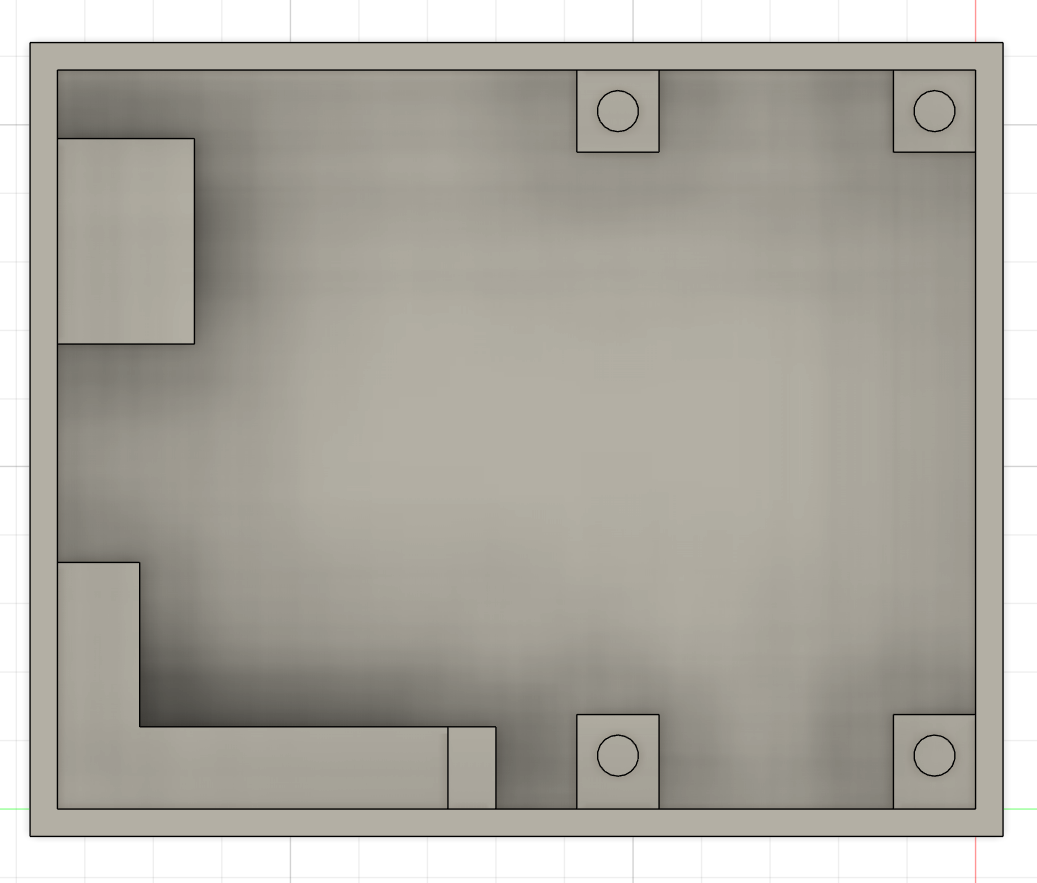
\includegraphics[scale=0.5]{/hardware/basis-draufsicht_fusion.png}
\caption{Draufsicht der Basis in AUTODESK Fusion}
\end{flushleft}
\end{figure}
\begin{figure}[H]
\begin{flushleft}
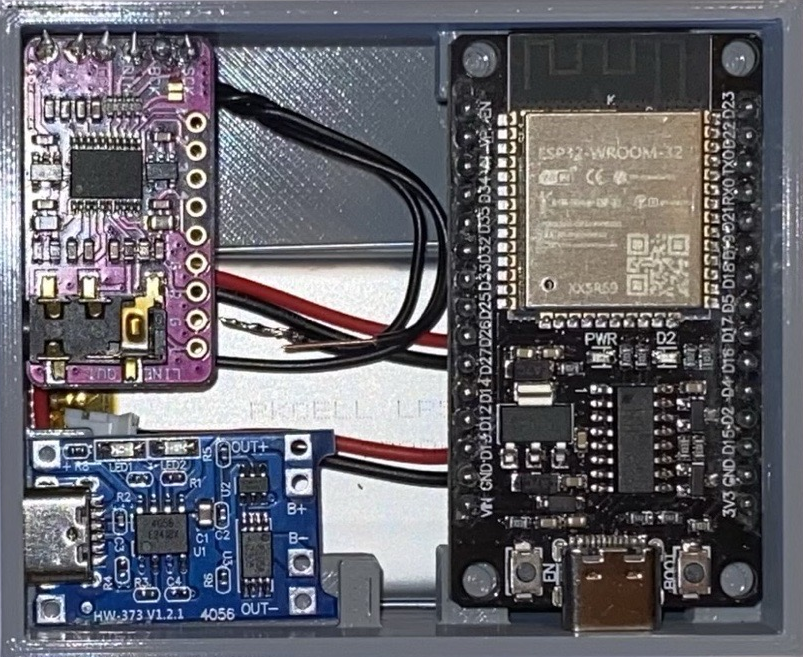
\includegraphics[scale=0.28]{/hardware/basis-inhalt_picture.png}
\caption{Bild der Basis mit den wichtigsten Komponenten an Ort und Stelle}
\end{flushleft}
\end{figure}
\noindent \textbf{Deckel} \newline
Der Deckel des Adapters ist grundsätzlich, wie die Wände der Basis, 71x58x2mm groß. Dieser hat jedoch eine zentrierte 67x54x1mm große Stufe. Mit dieser Stufe lässt sich der Deckel kleberlos auf den Adapter setzen und hält aufgrund der Eigenschaften des 3D-Drucks auch, zumindest für den Prototypen, fest genug.
Wie schon erwähnt, wird der DAC durch eine herabstehende Wand zusätzlich gestützt. Die Maße dieser Wand sind 32x2x10mm. Es würde keinen Sinn machen, die Wand wie beim Laderegler von der Außenwand aus überhängend zu machen, da der DAC länger als der Laderegler ist und die Buchse sich eher mittig in der entsprechenden Außenwand der Basis befindet.\newline
An der freien Seite der Stützwand (nicht die des DAC) befindet sich ein runder Schacht für die RGB-LED mit 5mm Durchmesser und eine Aussparung für den Aufsatz des Tasters mit 10,10mm Durchmesser. Der Taster mit den Grundmaßen 6x6mm wird durch eine Art U-Form aus Wänden im Gehäuse gehalten. Eine Wand davon bildet die gerade eben beschriebene Stützwand. Die untere Wand, auf der der Taster aufliegt, hat zudem zwei auf den Taster angepasste, 1mm große Aussparungen für die zwei Pole des Tasters.\newline
Wenn man in der Draufsicht auf den Deckel schaut, ist dort wo sich der Prozessor selbst befindet, ein Gitter in den Deckel eingelassen. Dieses Gitter hat die Maße 19,9x21,6mm, was etwas größer als der Prozessor des ESP32 ist. Das Gitter besteht aus diagonalen Streben, die jeweils 1,5mm breit sowie 1,5mm weit voneinander entfernt sind. So entsteht eine einfache und stabile Möglichkeit, Wärme durch den Deckel abzuleiten.\newline
\begin{figure}[H]
\begin{flushleft}
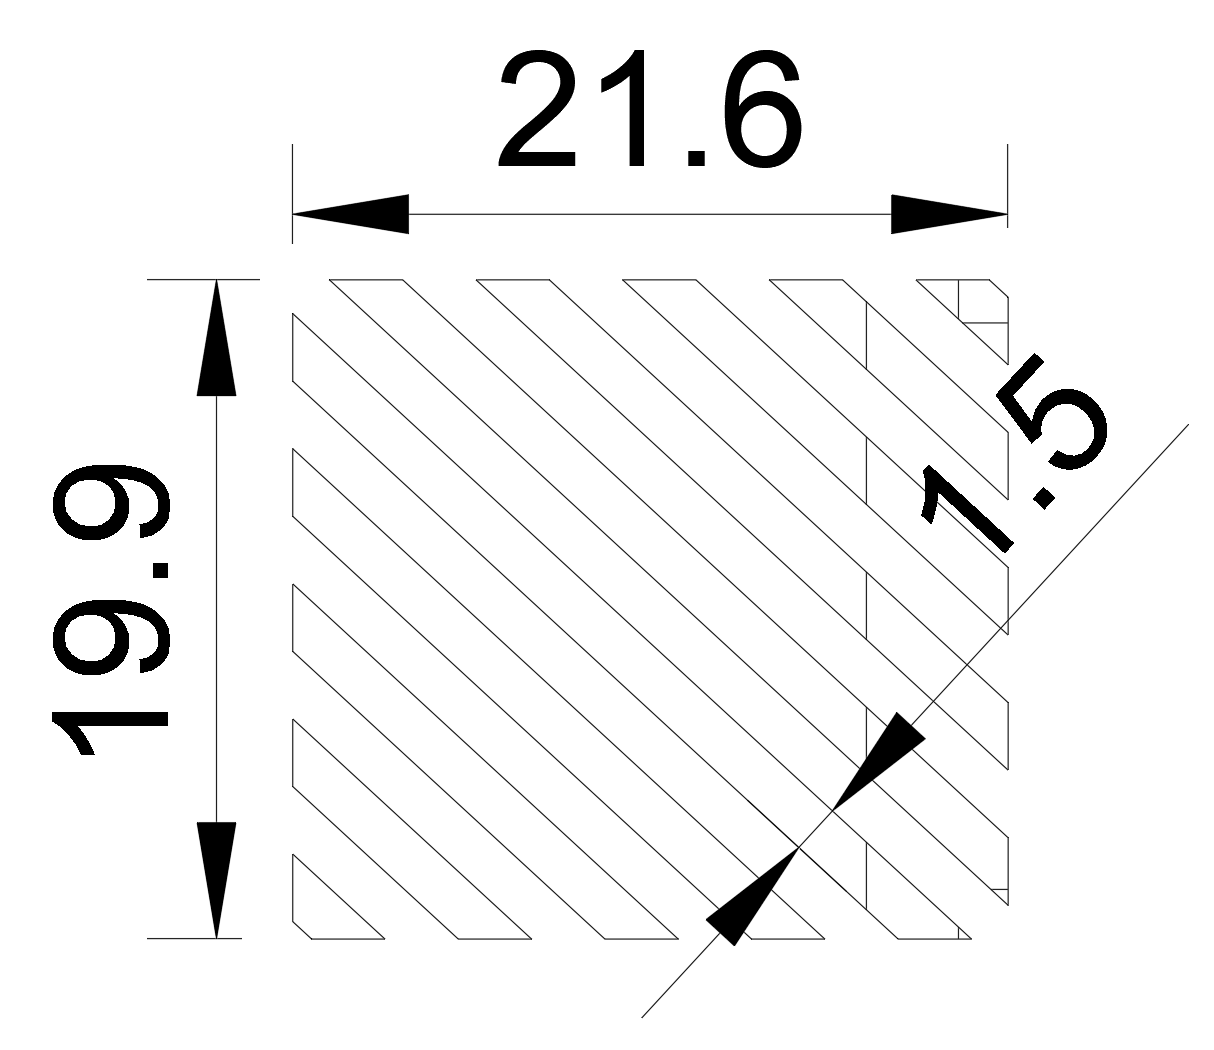
\includegraphics[scale=0.3]{/hardware/gitter-schema_fusion.png}
\caption{bemaßte Skizze des Belüftungsgitters in AUTODESK Fusion}
\end{flushleft}
\end{figure}
\noindent \textbf{Tasteraufsatz} \newline
Den Tasteraufsatz bildet ein Zylinder mit 9,5mm Durchmesser, auf dem sich ein weiterer Zylinder mit 5,5mm Durchmesser und zentrierter 3,5mm Aussparung für den Taster befindet.
\vspace{4mm}\newline
\parencite[vgl.][]{noauthor_urlnl12_nodate}\newline
\parencite[vgl.][]{noauthor_urlnl17_nodate}

\subsection{Fertigung Adaptergehäuse}
Das Material unseres Gehäuses wurde auf Kunststoff begrenzt. Für die Fertigung von Kunststoffgehäusen gibt es hauptsächlich diese Möglichkeiten (in diesem Fall kommt mangels Alternativen nur der 3D-Druck in Frage): 
\vspace{4mm}\newline
\textbf{Spritzgießen} \newline
\glqq Beim Spritzgießen wird der Kunststoff aus einem Plastifiziergerät (erwärmt den Kunststoff auf Schmelztemperatur) in einen Hohlraum (Formwerkzeug) gespritzt, in welchem er erst verdichtet wird und dann erkaltet.\grqq \newline 
Ein Vorteil für dieses Verfahren ist, dass auch komplizierte Formteile voll automatisiert sehr schnell in hohen Stückzahlen produziert werden können.
Der große Nachteil sind jedoch die hohen Stückkosten für die Formwerkzeuge.\vspace{4mm}\newline 
\parencite[vgl.][]{noauthor_urlnl14_nodate}
\vspace{4mm}\newline
\textbf{3D-Druck} \newline
Die zwei gängigsten 3D-Druck-Methoden sind Filament und Resin (Harz). Aufgrund des hohen Aufwands, den ein Resin-Drucker mit sich bringt, wurde für dieses Projekt die Methode mit Filament gewählt. \newline
Beim 3D-Drucken durch Fused Deposition Modeling (Schichtschmelzverfahren) wird Kunststoff in Drahtform (Filament) (die häufigsten Dicken sind 2,85mm (allgemein als 3mm bezeichnet) und 1,75mm wobei die 1,75mm Version weltweit am häufigsten verbreitet ist) durch beheizte Düsen geleitet und somit geschmolzen. Das nun weiche Filament wird in Schichten auf die Druckplatte aufgetragen und erhärtet kurz darauf. Durch dieses Schichten lassen sich präzise Körper aus Kunststoff bauen.
\vspace{4mm}\newline
\parencite[vgl.][]{noauthor_urlnl15_nodate}\newline
\parencite[vgl.][]{noauthor_urlnl16_nodate}

\subsubsection{Drucken des Prototypen}
Die Gehäuse-Prototypen wurden mit einem \glqq PRUSA MK4S\grqq{} 3D-Drucker gefertigt. Alle FFF-Drucker von Prusa sind grundsätzlich für 1,75-Filament konfiguriert.
\vspace{4mm}\newline
\textbf{Druckeinstellungen} \newline
Die Temperatur der Build Plate lag bei uns Standartmäßig auf 60°C. Die Drucktemperatur, also die der Nozzle (Düse) lag bei etwa 185°C. \newline
Das erste Layer wurde mit 0,15mm Dicke gedruckt, die restlichen mit 0,2mm Dicke. \newline
Als Infill-Pattern wurde \glqq Grid\grqq{} mit 20\% Dichte und 4mm Line-Distance gewählt. \newline
Das Drucken verlief mit den von uns gewählten Einstellungen reibungslos, jedoch an manchen Stellen etwas unsauber. Beispielsweise war das Ergebnis der Aussparung für den Taster im Deckel des Adapters so ungenau, dass der Durchmesser des Aufsatzes für den Taster um 0,5mm verkleinert werden musste. Sonstige Ungenauheiten stellten, zumindest abgesehen von der Optik, kein Problem dar. \newline
Man darf auch nicht vergessen, dass gewisse Drucke (Gehäusedeckel und -basis) Stützstrukturen erfordern. Stützstrukturen sind Konstruktionen, die der Drucker zur Unterstützung stark überhängender oder freischwebender Strukturen druckt. Jedoch sind diese nur temporär. Da das Stützmaterial nicht so fest an der Druckfigur haftet, wie die Teile der Figur selbst, kann es nach dem Druck mit einer herkömmlichen Zange entfernt werden. Diese Stützstrukturen lassen sich in der Slicer-Software genau einstellen und konfigurieren. So kann man unter anderem sicherstellen, dass das Entfernen einfach möglich ist und die Stützstruktur die Figur selbst nicht all zu stark beeinflusst.
\vspace{4mm}\newline
\parencite[vgl.][]{noauthor_urlnl16_nodate}
\subsection{Zusammensetzen des Prototypen}
Die Komponenten werden jeweils einzeln direkt mit dem Mikrocontroller verbunden. Bei diesem Prototyp lässt sich der Mikrocontroller nämlich vorerst als Platine betrachten, welcher zusätzliche Komponenten zugefügt werden.
\subsubsection{Schaltplan}
Die Verdrahtung zwischen den Komponenten und dem Mikrocontroller ist folgendermaßen gelöst:
\vspace{4mm}\newline
\textbf{Digital-/Analogwandler} \newline
BCK (Wandler) an D26 (Mikrocontroller)\newline
LCK (Wandler) an D25 (Mikrocontroller)\newline
DIN (Wandler) an D22 (Mikrocontroller)\newline
\vspace{4mm}\newline
\textbf{Taster} \newline
1 (Taster) an 3V3 (Mikrocontroller)\newline
2 (Taster) an D12 (Mikrocontroller)\newline
\vspace{4mm}\newline
\textbf{RGB-LED} \newline
R (LED) an D15 (Mikrocontroller)\newline
G (LED) an D2 (Mikrocontroller)\newline
B (LED) an D4 (Mikrocontroller)\newline
GND (LED) an GND (Mikrocontroller)\newline
\subsubsection{Verdrahten}
Bei unserem Prototypen wurden alle Komponenten, der Pinbelegung entsprechend, mit dem Mikrocontroller verbunden. Dabei kamen Drahtkabel, Litzenkabel und Steckkabel (herkömmliche Jumper Kabel) zur Verwendung. Dies hatte hauptsächlich den Grund, dass zum Beispiel nur mit Drähten nicht alle Verbindungen optimal möglich gewesen wären. Das ist hauptsächlich der Löthaftung an einigen Komponenten geschuldet. Um keine Wackelkontakte, oder gar unterbrochene Verbindungen zu riskieren, wurde für jede Verbindung einzeln entschieden, welches der genannten Verfahren sich am besten eignet. So entstanden zum Beispiel Steckverbindungen, gelötete Drahtverbindungen oder Mischungen aus gelöteten Litze- und Steckverbindungen (jeweils am anderen Ende des Kabels).
\vspace{4mm}\newline
\textbf{Löten}\newline
\glqq Das Löten ist das Verbinden von Metallteilen durch eine Metalllegierung (das Lot) unter Einfluss von Wärme/Hitze.\grqq{} \newline
Man unterscheidet grundsätzlich zwischen Weich- und Hartlöten. Ausschlaggebend dabei ist die Schmelztemperatur des Lots. So haben Weichlote eine Schmelztemperatur unter 450°C während Hartlote erst ab 450°C bis etwa 1100°C schmelzen. \glqq Das Weichlot wird verwendet, wenn die Verbindung zweier Metalle dicht und Leitfähig sein soll und um die mechanische Belastbarkeit keine hohe Anforderung gestellt wird.\grqq{} Da die in diesem Projekt benutzten Bauteile jedoch keine höheren Temperaturen vertragen, war Weichlöten für dieses Projekt die einzige Wahl. \newline
Um einen Lötvorgang aus eigener Erfahrung möglichst kurz zu beschreiben:\newline
Man hat beispielsweise zwei Kabel die man verbinden möchte und die Verbindung sollte möglichst fest halten und gut leiten. Zuerst müssen die Enden der Kabel abisoliert werden. Es kann helfen, wenn man die Enden schon vor der eigentlichen Verbindung sozusagen etwas \glqq verzinnt\grqq{}. Nun richtet man die Kabel zueinander so aus, wie sie später fixiert sein sollen. Man fährt mit dem Ende des Lots (umgangssprachlich Lötzinn) an die heiße Spitze des Lötkolben und schmilzt so etwas Lot auf die Verbindungsstelle (nicht zu viel, sonst erhält man dicke Tropfen; jedoch auch nicht zu wenig, da die Verbindung dann möglicherweise nicht ausreichend hält). Nach dem abkühlen macht es Sinn, die Lötverbindung durch leichtes rütteln oder ziehen zu überprüfen. Löten ist letztendlich aber ein Handwerk, das für saubere Ergebnisse Geduld und Übung vorraussetzt.
\vspace{4mm}\newline
\parencite[vgl.][]{noauthor_urlnl13_nodate}
\subsubsection{Kleben}
Damit alle Komponenten und Teile sicher im Gehäuse sitzen und nichts klappert oder sich gar bewegt, worunter die Lötverbindung leiden würde, müssen gewisse Komponenten angeklebt werden. Vorallem bei den Buchsen ist eine feste Verbindung wichtig, da diese bei jedem Ein- und Ausstecken großer Belastung ausgesetzt sind. Somit wurden der Laderegler und der Digital-/Analogwandler an den dafür gedruckten Stützen angeklebt. Zudem wurde der gedruckte Aufsatz in Gehäuseoptik für den Taster auf diesem befestigt. Für alle Klebverbindungen im Adapter wurden entweder herkömmliches Cyanacrylat (Superkleber) oder Schmelzklebstoff (Heißkleber) verwendet.

\section{Testen und Fehlerbehebung}
\subsection{Testen des Gesamtsystems}
\subsubsection{Testen des Prototypen}
Es gibt unzählbar viele Möglichkeiten einen Prototypen auf Herz und Nieren zu testen. Diese Diplomarbeit beschränkt sich jedoch auf einige wesentliche Aspekte wie Verarbeitung, Funktion und Useability.
\vspace{4mm}\newline
\textbf{Verarbeitung}
\vspace{4mm}\newline
Positives:\newline
Die äußere Verarbeitung des Multi Room Sound-Adapters ist für einen Prototypen sehr gut ausgefallen. Fertig zusammengesetzt wirkt das Gerät stabil und wertig. Es hat etwas Gewicht und nichts klappert wenn man es schüttelt. Die Buchsen halten der für Buchsen gemäßen Belastung stand. Beide der Buchsen lassen sich problemlos benutzen, beim Ein- und Ausstecken gibt es keine Probleme. Der Taster des Adapters ist, zumindest unseren Erwartungen nach, besonders gut ausgefallen, er hat ein angenehmes Klickfeeling und lässt sich reibungslos betätigen. Die Statusanzeige funktioniert so wie sie soll.
\vspace{4mm}\newline
Negatives:\newline
Man sieht dem Gehäuse bei guter Beleuchtung eindeutig an, dass es 3D-gedruckt wurde. Manche Oberflächen wirken eher geriffelt als flach. Diese Oberflächeneigenschafen sind völlig normal für 3D-Drucker und beeinflussen die Funktionsweise des Gesamtsystems kaum. Bei einem tatsächlichen Vetrieb des Produkts müsste man sich jedoch noch einmal genau über Herstellungsmöglichkeiten für kleinere Gehäuse informieren oder das Gehäuse, wie auch bei der Auswahl des Fertigungsverfahrens schon kurz diskutiert, einfach Spritzgießen lassen. Ein Spritzguss hat bessere Oberflächeneigenschaften als ein 3D-Druck.
\vspace{4mm}\newline
\parencite[vgl.][]{redaktion_urlnl18_2020}
\vspace{4mm}\newline
\textbf{Funktion}\newline
Der Adapter funktioniert und erfüllt seine Funktionen ohne Fehler oder Komplikationen.
\vspace{4mm}\newline
\textbf{Usability}\newline
Die Anwendung des Adapter ist grundsätzlich angenehm. Es gilt jedoch zu bedenken, dass uns sowohl Software als auch Hardware schon bekannt sind. Wie sich die Usability verändert, wenn der Adapter von jemandem benutzt wird, der ihn noch nie gesehen hat, kann man nur schlecht sagen. Dafür wären mehrere Produkttests nötig. Falls ein Vetrieb des Produkts in betracht gezogen werden würde, wäre dies auf jeden Fall ein wichtiger Punkt.\newline
\subsection{Auftretende Fehler beheben}
Es handelt sich hierbei nicht direkt um einen Fehler, jedoch ist uns wichtig, dass auch die Optik des Gehäuse so gut wie möglich ausfällt. Deshalb wurde viel mit verschiedenen Tricks und Methoden gearbeitet, die 3D-Drucke wertiger ausfallen zu lassen.\newline
So war anfangs beispielsweise die Druckgenauigkeit in Millimeter nicht auf dem kleinst-möglichen Wert, was für Testdrucks aufgrund der wesentlich kürzeren Druckzeit jedoch völlig in Ordnung ist. Wenn alles passt, macht es aber definitiv Sinn eine lange Druckdauer in Kauf zu nehmen, um das für den vorliegenden 3D-Drucker genauste Ergebnis zu erhalten.\newline
Eine Herausforderung war die Beschriftung des Deckels. Diese war beim ersten Testdruck teilweise unlesbar ungenau. Das der \glqq Boden\grqq{} der Schrift auf Grund des druckabhängigen Überhanges (die größte Fläche also die Oberseite des Deckels muss praktisch auf der Druckplatte sein) nicht glatt wird, war uns klar. Jedoch hatte dieses Erscheinungsbild augenscheinlich nichts mit dem Überhang zu tun. Bei genauerem Betrachten fiel auf, dass das erste Layer fast wie gepatzt aussah. Ein weiterer Versuch mit simpler Schriftart und bei dem lediglich die Druckgenauigkeit des ersten Layers von 0.15 auf 0.1, die der restlichen Layer von 0.2 auf 0.15 kalibriert wurde, zeigte jedoch schon für einen 3D-Druck schöne Ergebnisse.\newline
Eine weitere Möglichkeit zum glätten der schon zuvor beschriebenen riffelartigen Oberflächen ist sogenanntes Ironing. \glqq Ironing beschreibt die einstellbare Funktion in einiger Slicer-Software. Ironing bietet dir die Möglichkeit, die letzte 3D-Druckschicht mit der Nozzle zu "bügeln". Die Nozzle deines 3D-Druckers bewegt sich ohne dabei zu extrudieren nochmals über die zuletzt gefertigte Schicht. Durch diesen Vorgang glättet sie die Objekt-Oberfläche. Du bekommst somit eine verbesserte und glatte letzten Schicht.\grqq{} Beim PRUSA MK4S war diese Funktion sehr zufriedenstellend. Oberflächen werden, ohne den gesamten Druck zu beeinflussen, glatter.\newline
\vspace{4mm}\newline
\parencite[vgl.][]{noauthor_urlnl19_nodate}
\newpage
\section{Schluss}
\subsection{Konklusion Hardware}
Ziel des Hardware-Teils in dieser Diplomarbeit war es, passende Komponenten zu finden und diese in einem selbst designten Gehäuse zu einem Prototypen des MAA zusammenzusetzen. Dies wurde, wie geplant, umgesetzt. Dabei kamen grundlegende Methoden wie 3D-Design, 3D-Druck, Löten und weitere zum Einsatz. Grundsätzlich lief alles wie geplant, es ergaben sich jedoch öfters größere Herausforderungen dort, wo man eigentlich keine erwartete. Für diese fand sich aber immer eine passende Lösung.
\subsection{Konklusion Software}
Abschließend kann man sagen, dass das Ziel, eine funktionierende Software für den Adapter sowie eine funktionierende Smartphone-App im Zuge der Diplomarbeit zu entwickeln, erfüllt wurde. Das heißt aber nicht, dass der Code dieser beiden Applikationen fertiggestellt ist. Wie bereits beschrieben können in Zukunft bei noch zahlreiche neue Features für die Applikationen entwickelt werden, welche ansonsten den Rahmen der Diplomarbeit gesprengt hätten.
\newpage
\section{Einzelnachweise}
\subsection{Literaturverzeichnis}
\printbibliography
\newpage
\subsection{Abbildungsverzeichnis}
\listoffigures
\subsection{Tabellenverzeichnis}
\listoftables
\newpage
\subsection{Anhang}
\subsubsection{Code Mikrocontroller}
\subsubsection{Code Smartphone-App}
\end{document}
